%Concerns:
%Need to fix citation 24 from running to papers edge.

\documentclass[conf]{new-aiaa}
%\documentclass[journal]{new-aiaa} for journal papers
\usepackage[utf8]{inputenc}

\usepackage{graphicx}
\usepackage{caption}
\usepackage{subcaption}
\usepackage[table,x11names]{xcolor}
\usepackage{array}
\usepackage{amsmath}
\usepackage[version=4]{mhchem}
\usepackage{siunitx}
\usepackage{longtable,tabularx}
\usepackage{float}
\usepackage{rotating}
\usepackage{makecell, multirow}
\floatstyle{plaintop}
\restylefloat{table}
\setlength\LTleft{0pt} 


\title{Guidance, Navigation, and Control Subsystem Design for ABEX Satellite}

\author{Maxwell Cobar\footnote{Graduate Research Assistant, AIAA Student Member.}, Andrew Givens\footnote{Graduate Research Assistant, AIAA Student Member.}, Caroline Franklin\footnote{Undergraduate Research Assistant, AIAA Student Member.}\\ William Sherman\footnote{Undergraduate Research Assistant, AIAA Student Member.}, Wei Min Patrick\footnote{Undergraduate Research Assistant, AIAA Student Member.}, Aaron Godfrey\footnote{Undergraduate Research Assistant, AIAA Student Member.} and Carlos Montalvo\footnote{Associate Professor, AIAA Senior Member.}}
\affil{William B. Burnsed Jr. Deparment of Mechanical, Aerospace and Biomedical Engineering\\ College of Engineering\\University of South Alabama \\150 Student Services Dr. Mobile, AL, 36688}

\begin{document}

\maketitle

\begin{abstract}
This paper details the design of the Guidance, Navigation and Control (GNC) Subsystem for the Alabama Burst Energetics Explorer (ABEX) Satellite. This satellite will be used to measure Gamma Ray Bursts in Low Earth Orbit. Although the GNC subsystem has relatively benign constraints, the program has seen numerous design changes requiring the need for quick GNC design. As such, an analysis tool was created to help with the sizing of the reaction wheels and magnetorquers. In addition, an under-actuated control law is being developed as a means of attitude control for the satellite and reaction wheel desaturation capability during the life of the satellite while only using a two axis control actuator. The results from the analysis tool are shown and were considered during the design process. The derivation for the under-actuated control law is shown to be a viable solution however further simulation is required to ensure robustness.
\end{abstract}

%%%%%%%%%%%%%%%%%%%%%%%%%%%%%%%%%%%%%%%%%%%%%%%%%%%%%%%%%%%%%%%%%%%%%%%%%%%%%%%%%%%%%%%%%%%%%%%

\section{Nomenclature}
{\renewcommand\arraystretch{1.0}
\begin{longtable*}{@{}l @{\quad=\quad} l@{}}
$ABEX$  & Alabama Burst Energetics Explorer \\
$ADCS$  & Attitude Determination and Control Subsystem \\
$C\&DH$ & Command and Data Handling \\
$CONOPS$  & Concept of Operations \\
$DOF$  & Degrees of Freedom \\
$DSN$  & Deep Space Network \\
$ECI$ & Earth Centered Inertial \\
$FEEP$ & Field-Emission Electric Propulsion \\
$FOV$ & Field of View \\
$GSN$  & Ground Station Network \\
$GNC$  & Guidance, Navigation, and Control \\
$GPS$  & Global Positioning System \\
$HEO$  & High Earth Orbit \\
$LEO$  & Low Earth Orbit \\
$ID$  & Interface Diagrams \\
$IGRF$  & International Geomagnetic Reference Field \\
$IMU$  & Inertial Measurement Unit \\
$MarCO$  & Mars Cube One \\
$MRD$  & Magnetic Resonance Dipole \\
$RCS$ & Reaction Control System \\
$RK$ & Runge-Kutta Integration\\
$RW$ & Reaction Wheel \\
$SRP$  & Solar Radiation Pressure \\
$SS$  & Sun Sensors \\
$STLC$  & Small-Time Locally Controllable \\
$TBD$  & To Be Determined \\
$UR$  & Upon Request \\
$TPM$  & Technical Performance Metrics \\
$WMM$  & World Magnetic Model \\
$ECI$  & Earth Centered Inertial Frame \\
$NDA$ & Non-Disclosure Agreement \\
$BCT$ & Blue Canyon Technology
\end{longtable*}}

%%%%%%%%%%%%%%%%%%%%%%%%%%%%%%%%%%%%%%%%%%%%%%%%%%%%%%%%%%%%%%%%%%%%%%%%%%%%%%%%%%%%%%%%%%%%%%%
\section{Introduction}
CubeSats and NanoSats are often characterized as small satellites found in low or medium Earth orbit \cite{1}. Although this is true for most, recent advancements in miniaturized technologies and reduced cost have fostered a new wave of deep space missions involving CubeSats. NASA’s MarCO interplanetary nano spacecraft mission in May of 2018, was one of the first to shed light on the possibilities of small satellite utilization and helped foster the development of technologies to specifically address the challenges that a CubeSat’s small volume brings. Opportunities such as piggybacking, where small satellites are launched as secondary payloads on larger missions, have solved the issue of getting to an intended destination \cite{2}. On the other hand, once the satellite is ejected, relying solely on what is housed within its small three-dimensional footprint is an entirely new challenge.

Escaping the relative safety of low Earth orbit (LEO) and the Earth’s magnetosphere, CubeSats venturing into deep space will face the same hostile environment as their larger, more capable counterparts. Issues with power, thermal management, guidance, navigation, control, propulsion, and so on are exacerbated by the environment and pose a serious threat to mission feasibility when considered with the limited mass and volume budget of these spacecrafts \cite{3,4}. The Attitude Determination and Control System (ADCS) is one that is particularly limited by this mass and volume restriction. Composed of sensors, actuators, and computational hardware, depending on the systems design, the ADCS can constitute a large portion of the satellite's mass and volume budget. This is especially true in the case of systems requiring redundant, or secondary, actuation such as reaction wheels (RWs), magnetorquers, and reaction control thrusters (RCS). According to Xia [5], from 2003 to 2017, 54\% of successfully launched CubeSats utilized a reaction wheel-based attitude control scheme with the second most popular scheme being passive magnetic at 17\%. 

Although RWs are well suited for small satellites because of their relative performance for a given size \cite{5}, they do also come with their own set of problems, mainly consisting of control saturation. This requires secondary actuation to apply an external torque relative to the wheel itself to counteract the torque created by slowing down the wheel. In LEO, desaturization can occur through the use of magnetorquers. However, in deep space or high Earth orbits (HEO), this is usually accomplished by thrusters, a costly commodity in terms of volume and mass. Combining a three axis RCS system with a primary propulsion system for station keeping would most likely overwhelm the mass, volume, and power budget of a small satellite.

An even more worrisome factor in this case is that of actuator failure. In the case of a RW failure or a thruster failure, the system would then become underactuated with fewer functional RWs than principal axes \cite{6,7}. Thus, the utilization of an underactuated control law allows for an actuartor failure to occur and still provides the system with adequate control authority.  Underactuated systems can also be by design to reduce mechanical complexity and cost.

In either case, the difficulty in controlling this type of system arises from the inability for the dynamics to be stabilized by any smooth or continuous time-invariant feedback law due to the equations of motion violating Brockett's necessary condition. This is even the case if the system is small time locally controllable (STLC) \cite{7}. Control laws for time-invariant fully actuated systems are well understood at this point \cite{8}, but the complexity of the underactuated state has not had the same level of analysis. That being said, numerous past works have developed control laws for such complex systems, especially in terms of attitude stabilization, with first analysis of the equations of rotational motion being addressed for rigid bodies with one, two, and three control torques in \cite{9}. Underactuated control detumbling has been addressed, although it is with the application of one magnetorquer which takes advantage of a non-constant magnetic field when in an inclined orbit \cite{10}. According to Horri and Hodgart, underactuated reaction wheel control is proposed based on Rodriguez parameterization of the attitude, although it is noted that initial angular momentum must be small or otherwise accounted for by magnetorquers  \cite{11}. In previous studies, discontinuous feedback control methods are discussed and point to nonsymmetric inertia matrices and suggest that the attitude dynamics are accessible if, and only if, the uncontrolled principal axis is not an axis of symmetry \cite{12,13}. The non-diagonal nature of the satellite’s inertia matrix allows the cross products of inertia to transfer momentum from the uncontrolled axis to those that are controlled. Although detumbling is addressed, little to no previous work has been done on applying this to momentum dumping. 

%%WILLLIAM SHERMAN DO NOT UPDATE THE NEXT TWO PARAGRAPHS

This report specifically explores the GNC system for the Alabama Space Grant Consortium’s (ASGC) Alabama Burst Energetics Explorer (ABEX) Satellite which will detect gamma-ray burst over the course of 1 year. The satellite will utilize piggybacking to get into LEO. During initial design, the orbit was to be highly elliptical with a perigee of 160 km and an apogee of 60,000 km (well outside the Global Position System (GPS)). Given this low perigee and high apogee, design trade offs for attitude control were made. Magnetorquers are effective in the low altitude portion of the orbit but ineffective at high altitudes. Furthermore, the main propulsion system only provides two axis control (pitch and yaw) and thus, if the primary propulsion mechanism is to be used to de-saturate reaction wheels as opposed to magnetorquers, an underactuated control law must be utilized. A new control approach specifically addressing underactuated reaction wheel momentum dumping maneuvers is proposed here as well. The controller falls under the category of a nonlinear, Lyapunov-based, feedback controller using local representation of attitude as suggested by Peterson \cite{7}. Numerical simulations are offered as well as the controller derivation to prove feasibility. 

After considerable design changes by the System Engineering team, the orbit was changed to a 600 km sun synchronous orbit given launch vehicle constratins. The propulsion mechanism was also removed and thus station keeping can be moved to Reaction Wheels and Magnetorquers. Although the orbit and subsequently the requirements have changed drastically, the analysis tool was able to easily update the performance of the GNC subsystem. The two axis control law although not needed is still included in this report given the novel approach to two axis control.

%%%%%%%%%%%%%%%%%%%%%%%%%%%%%%%%%%%%%%%%%%%%%%%%%%%%%%%%%%%%%%%%%%%%%%%%%%%%%%%%%%%%%%%%%%%%%%%

\section{Attitude Determination and Control Subsystem Overview}

The main responsibilities of the ADCS are to estimate its attitude and position, detumble the spacecraft during release and control the satellite to a desired attitude. The ADCS will use a combination of sensors to obtain full state feedback of the spacecraft including position and orientation. Furthermore, some control mechanism is required to point the satellite to a desired orientation.

\subsection{Requirements}

The ADCS is one subsystem of the larger satellite system of interest. This program is in collaboration with four other universities in Alabama coordinated by ASGC. Thus, the Systems Engineering team currently located in the University of Alabama Huntsville (UAH) dictated the requirements for the ADCS. Table \ref{t:SYS_REQ} shows the subsystem requirements for the ADCS. Green rows indicate that the design satisfies the requirements while yellow rows indicate that the status of the requirement is still pending due to an NDA with Blue Canyon Technologies (BCT). In this case, most requirements have been met while the sensor mass, location accuracy, and attitude control sensitivity must still be negotiated with the Systems Engineering team and BCT.

\begin{center}
\begin{longtable}[c]{|c|c|p{4.0cm}<{\centering}|c|}
\caption{GNC System Requirements} \label{t:SYS_REQ} \\

\hline \rowcolor{cyan} \multicolumn{1}{|c|}{\textbf{ID}} & \multicolumn{1}{c|}{\textbf{Name}} & \multicolumn{1}{c|}{\textbf{Text}} & \multicolumn{1}{c|}{\textbf{TPM}} \\ \hline 
\endfirsthead

\multicolumn{4}{c}%
{{\bfseries \tablename\ \thetable{} -- Continued from previous page}} \\
\hline \rowcolor{cyan} \multicolumn{1}{|c|}{\textbf{ID}} & \multicolumn{1}{c|}{\textbf{Name}} & \multicolumn{1}{c|}{\textbf{Text}} & \multicolumn{1}{c|}{\textbf{TPM}} \\ \hline 
\endhead

\hline \rowcolor{cyan} \multicolumn{4}{|r|}{{\textbf{Continued on next page}}} \\ \hline
\endfoot

\hline \hline
\endlastfoot

\rowcolor{yellow} A.SYS.7.2  & Attitude Control Sensitivity & The attitude control sensitivity shall be of smaller or equal to 0.2 deg/s per axis & NDA BCT\\ \hline 
\rowcolor{yellow} A.SYS.7.4  & Location Accuracy & The s/c shall be able to calculate its position +/- 1,000 km & NDA BCT\\ \hline 
\rowcolor{green} A.SYS.7.5  & Attitude Knowledge & The s/c shall be able to determine its attitude +/- 1 deg/axis & 0.05 deg\\ \hline 
\rowcolor{green} A.SYS.7.6  & Reaction Wheel Mass & The sum of the mass of the reaction wheels shall not exceed 1,182.5 grams & 1.0 kg\\ \hline
\rowcolor{yellow} A.SYS.7.7  & Sensor Mass & The sum of the mass of the attitude determination sensors used shall be less than 500 grams & NDA BCT\\ \hline 
\rowcolor{green} A.SYS.7.8  & Reaction Wheel Volume & The sum of the volumes of the reaction wheels shall be smaller than 767.8 cm$^{3}$ & 367.5 cm$^{3}$\\ \hline 
\rowcolor{green} A.SYS.7.9  & Attitude Sensor Volume & The sum of the volume for the attitude sensors used for attitude determination shall be less than 520.3 cm$^{3}$ & 500 cm$^{3}$\\ \hline 
\rowcolor{green} A.SYS.7.12  & Tipoff Recovery & The s/c shall recover from an initial angular velocity up to 10 deg/s with inertia per axis [0.507,0.441,0.332] kg.m$^{2}$ & $\sim$3 orbits\\
\end{longtable}
\end{center}


%This table is poorly made and rigged together with fucking scotch tape.
%Tables are a fucking nightmare.https://www.overleaf.com/project/60b7eaa68d972e9212badaf7 God, I hate this.
%I hope you read these comments a laugh because I have died a little inside making this table.
%DO NOT MESS WITH THIS TABLE! Ask me (Maxwell) to edit this table.
%I read this and loled. Montalvo...
%Sorry I touched your table just a little...nothing personal just needed it to fit on page 3...Caroline
% \begin{table}[H]
% \centering
% \caption{GNC System Requirements}
% \begin{tabular}[t]{|c|c|c|c|}
% \hline
% \rowcolor{cyan} \textbf{ID} & \textbf{Name} & \textbf{Text} & \textbf{TPM} \\
% \hline
% \rowcolor{yellow} & & Attitude control sensitivity& \\
% \rowcolor{yellow} A.SYS.7.2& Attitude Control Sensitivity& shall be of smaller or& NDA BCT\\
% \rowcolor{yellow} & &  equal to 0.2 deg/s per axis& \\
% \hline
% \rowcolor{yellow} & & The s/c shall be able&\\
% \rowcolor{yellow} A.SYS.7.4& Location Accuracy& to calculate its position& NDA BCT\\
% \rowcolor{yellow} & & +/- 1,000 km&\\
% \hline
% \rowcolor{green} & & The s/c shall be able& \\
% \rowcolor{green} A.SYS.7.5& Attitude Knowledge& to determine its attitude& 0.05 deg\\
% \rowcolor{green} & & +/- 1 deg/axis& \\
% \hline
% \rowcolor{green} & & The sum of the mass of&\\
% \rowcolor{green} A.SYS.7.6& Reaction Wheel Mass& the reaction wheels shall& 1.0 kg \\
% \rowcolor{green} & & not exceed 1,182.5 grams&\\
% \hline
% \rowcolor{yellow} & & The sum of the mass of the attitude&\\
% \rowcolor{yellow} A.SYS.7.7& Sensor Mass& determination sensors used& NDA BCT\\
% \rowcolor{yellow} & & shall be less than 500 grams&\\
% \hline
% \rowcolor{green} & & The sum of the volume of the& \\
% \rowcolor{green} A.SYS.7.8& Reaction Wheel Volume& reaction wheels shall& 367.5 cm$^{3}$\\
% \rowcolor{green} & & be smaller than 767.8 cm$^{3}$& \\
% \hline
% \rowcolor{green} & & The sum of the volume for the attitude& \\
% \rowcolor{green} A.SYS.7.9& Attitude Sensor Volume& sensors used for attitude& 500 cm$^{3}$\\
% \rowcolor{green} & & determination shall be less than 520.3 cm$^{3}$ & \\
% \hline
% \rowcolor{green} & & The s/c shall recover from& \\
% \rowcolor{green} & & an initial angular& \\
% \rowcolor{green} A.SYS.7.12& Tipoff Recovery& velocity up to 10 deg/s& $\sim$3 orbits\\
% \rowcolor{green} & & with inertia per axis& 
 \\
% \rowcolor{green} & & [0.507,0.441,0.332] kg-m$^{2}$& \\
% \hline
% \end{tabular}
% \label{t:SYS_REQ}
% \end{table}
 
 \subsection{Block Diagram Definition}

Given the requirements of the ADCS, it is possible to create a block diagram definition of the overall architecture. Below is a graphic of block definition diagram. (See Figure \ref{fig:BDD}) The input to all of the hardware components is power and the output from all the various subsystems go to the Flight Control Board. The BDD is broken into 3 major subsystems: Attitude Estimation, Attitude Control, and Position Estimation. For Attitude Estimation, the 3DOF rate gyro outputs angular velocities in the body frame, the magnetometer outputs magnetic field direction and strength in the body frame, the star tracker outputs a full quaternion, and the sun sensor outputs the azimuth and elevation angles of the sun vector in the body frame. The Spice Library is a star catalogue developed by NASA’s Jet Propulsion Laboratory. The input to the Spice Library is the real-time from the ADCS Board as well as the latitude, longitude and altitude from the Position Estimation subsystem. The output from the Spice Library is a star catalogue to be used with the Star Tracker as well as an inertial sun vector based on the position of Earth which is computed via the real-time clock. The Magnetic Field Model will come from either the IGRF or MWW2020 model. The input for the Magnetic Field Model is the position of the satellite from the ADCS Board and the output is the magnetic field in the inertial frame. There are a few benefits to not using a sun sensor, including less power draw and an overall lighter system. There is also a smaller volume and mass penalty which would be financially beneficial. However, this configuration is the least redundant as the only way to obtain attitude would be to use the star tracker. Options with no Magnetometer were considered as well, however, magnetometers are also required for magnetorquer control laws and thus, if the magnetometer were removed, magnetorquers would need to be removed as well leading to this option being thrown out as well. An IMU is also a necessity since not having an IMU would violate requirement A.SYS.7.2 defined by the systems engineering team. For attitude control, magnetorquers and Reaction wheels were considered integral for the design. In this case, reaction wheels were necessary to achieve the attitude control sensitivity as defined by requirement A.SYS.7.2. No other control mechanism (magnetorquers or gimbaled thrusters) can achieve the necessary level of control. Thus, reaction wheels were included in each design. magnetorquers were only considered once the analysis tool revealed that torque rods of adequate size could desaturate RWs over the time span of a few orbits. In addition, the change to a LEO meant that magnetorquers were an obvious choice. Note that the gimbaled thruster was removed after the orbit had been changed. The requirement for 1000 km knowledge necessitates the inclusion of an RK4 integration loop in the event GPS and any Ground Station Network (GSN) does not update fast enough to obtain a sufficient level of precision. Thus, in between sensor updates, the position will need to be estimated using the RK4 integration. However, it may be possible to only use GSN or GPS.
The outputs of the GPS receiver are altitude, longitude, latitude, velocity, and GPS time. The input to the RK4 integration loop algorithm is the coordinates of the satellite from the ADCS Board, and the output from the RK4 integration loop algorithm is the time-updated coordinates of the satellite. Finally, the ADCS Board receives an output from the communication board. This output consist of range data that will be received from a GSN that can be used to obtain current position. Note that the reading from the GSN is not part of the BDD because it is part of the Communications subsystem. In addition, the command and data handling subsystem is not pictured although the C&DH subsystem is responsible for sending commands to the GNC subsystem.

\begin{figure}[H]
\centering
\includegraphics[width=1.0\textwidth]{Figures/BDD_GNC.png}
\caption{Block Definition Diagram of GNC Subsystem}
\label{fig:BDD}
\end{figure}




%%%%%%%%%%%%%%%%%%%%%%%%%%%%%%%%%%%%%%%%%%%%%%%%%%%%%%%%%%%%%%%%%%%%%%%%%%%%%%%%%%%%%%%%%%%%%%%

\section{Attitude Estimation}
\subsection{Attitude Estimation Overview}
Attitude estimation is the function by which the orientation of the vehicle is found within three-dimensional space. This requires estimation methods to obtain a full quaternion. Attitude estimation requires multiple sensors which may or may not include: 

\begin{enumerate}
\item Sun Sensors
\item Earth/Horizon Sensors
\item Star Trackers
\item Magnetometers
\item Rate Gyros
\end{enumerate}

Typically, utilizing a star tracker on its own will use an internal Quest algorithm with an on-board star catalog to produce a full quaternion. However, it is possible to obtain a full quaternion using a sun sensor and magnetometer. The sun sensor produces a body frame vector ($S_{b}$) and the magnetometer produces a body frame magnetic field vector ($B_{b}$). Using the IGRF/WMM2020 model will provide an inertially fixed magnetic field vector ($B_{i}$), assuming the position of the satellite is known. A sun ephemeris catalog, which will more than likely be the SPICE Library, will produce an inertial sun vector ($S_{i}$) \cite{SPICE}. The vectors ($S_{b}$ and $B_{b}$) can be used to create an orthonormal basis in the body frame. The same can be done for the inertial frame. Using both orthonormal bases, simple linear algebra techniques can be used to extract the quaternion from the transformation matrix.

The CONcept of OPerationS (CONOPS) for attitude estimation is shown in the following activity diagram. Figure \ref{fig:AE_AD} shows the attitude estimation from the start tracker, rate gyro and magnetometer. The attitude estimation starts by polling the rate gyro to get the angular velocity of the satellite. The algorithm then polls the magnetometer to get the direction and strength of the magnetic field in the body frame. Note the rate gyro and magnetometer measurements are for the attitude control B-dot control algorithm. Finally the star tracker is polled. If the quaternion from the star tracker is valid, the system moves on. If the star tracker measurement is not valid, the system moves to the Sun Sensor and Magnetometer estimation algorithm. The SS/MAG estimation algorithm works by using the already polled magnetometer measurement and then polling the sun sensor to find the azimuth and elevation angles of the sun in the inertial frame followed by the SPICE Library. The sun sensor angles are then converted to the body frame. The magnetic field model is polled next, followed by the IGRF Library. The International Geomagnetic Reference Field (IGRF) model gives the magnetic field direction and strength in the inertial frame, and the SPICE Library gives a sun vector that is converted to the Earth Centered Inertial (ECI) frame. Lastly, quaternion linear algebra is used to estimate the attitude of the satellite.

%Finally, Figure \ref{fig:AE_AD_3} shows CONOPS of the attitude estimation procedure. The CONOPS starts with getting the initial attitude estimation. This process is shown in Figure \ref{fig:AE_AD_1}. Next, Euler integration is used to integrate the rate gyro's measurements to obtain the orientation of the satellite. If the integration time is greater than the initial time, the process is paused until the integration time is no longer greater than the initial time. When this happens, the attitude is updated with a new estimation. This process is shown in Figure \ref{fig:AE_AD_1}. Lastly, if a new quaternion is found with the attitude estimation update then the Kalman Filter is updated. If no new quaternion is found, the process repeats by starting back at Euler integration of the rate gyro.

\begin{figure}[H]
\centering
\includegraphics[width=0.70\textwidth]{Figures/AE_AD.png}
\caption{Attitude Estimation Procedure}
\label{fig:AE_AD}
\end{figure}

\subsection{Sun Sensors and Sun Ephemeris Data}

Sun sensors operate by allowing thin beams of light to hit an array of photodetectors which induce a voltage. The direction of the sun can be determined by orienting two of these sensors perpendicular to one another. These voltage signals are sent through a database called the SPICE library which determines the Sun's position over time in spherical coordinates. Below (See Table \ref{t:SS}) is the list of viable sun sensor options where some prices are available upon request (UR). Note that these do not represent all sun sensors in the CubeSAT market, however after careful consideration, these three were the best options to choose from for this use case. Note that Blue Canyon Technologies has also been consulted as an option for Sun Sensors using their integrated subsystems.

\begin{table}[H]
 \centering
 \caption{Sun Sensor Options}
 \begin{tabular}[t]{|c|p{2.0cm}|c|c|c|p{1.5cm}|p{1.3cm}|c|}
    \hline
    \textbf{Model Number} & \textbf{Manufacturer} & \textbf{Mass (kg)} & \textbf{Volume (U)} & \textbf{Power (W)} & \textbf{Accuracy (deg)} & \textbf{FOV (deg)} & \textbf{Cost (\$)} \\
    \hline
    NFSS-411 \cite{NFSS-411} & NewSpace Systems & 0.035 & 2.18x10$^{-02}$ & 0.130 & 0.100 & 140 & UR \\
    \hline
    SSOC-D60 \cite{SSOC-D60} & SolarMEMS & 0.036 & 1.80x10$^{-02}$ & 0.315 & 0.300 & 60 & 14,400 \\
    \hline
    nanoSSOC-D60 \cite{nanoSSOC-D60} & SolarMEMS & 0.006 & 3.55x10$^{-03}$ & 0.076 & 0.500 & 60 & 4,300 \\
    \hline
\end{tabular}
\label{t:SS}
\end{table}

\subsection{Earth/Horizon Sensors}
Earth or horizon sensors operate by using a spinning mirror to focus light onto a sensing element called a bolometer. The device sweeps out the area of a cone and detects when the infrared signal from Earth is received then lost. This calculates the width of the earth which determines angle to the Earth. This, in conjunction with an Earth ephemerides table, can be used to obtain orientation. Initially, the highly elliptic orbit only put the satellite in LEO for approximately 20 minutes resulting in an Earth sensor would only be useful for a very short amount of time. As such, no Earth sensors were chosen and they were removed from the ADCS design. Once the orbit was changed from highly elliptic to LEO the option of using an Earth/Horizon sensor was reconsidered, but ultimately removed once the option of using an integrated subsystem from BCT became an option. The Earth/Horizon sensors were removed from contention to save mass, volume, and power.

\subsection{Star Trackers}
Star trackers measure the position of stars using a camera. These positions are put through a star catalog containing the known positions of stars typically via the QUESST algorithm \cite{cassidis}. Since the position of the stars is known, the satellite's attitude can be determined in reference. Below (See Table \ref{t:ST}) constitutes the top two star trackers chosen for ABEX.

\begin{table}[H]
 \centering
 \caption{Star Tracker Options}
 \begin{tabular}[t]{|c|c|c|c|c|p{1.3cm}|p{1.4cm}|}
    \hline
    \textbf{Model Number} & \textbf{Manufacturer} & \textbf{Mass (kg)} & \textbf{Volume (U)} & \textbf{Power (W)} & \textbf{Accuracy (deg)} & \textbf{FOV (arcsec)} \\
    \hline
    ST 200 \cite{ST-200} & Berlin Space Tech & 0.106 & 2.08x10$^{-01}$ & 0.67 & 10 & 40 \\
    \hline
    ST 200 \cite{ST-200H} & Hyperion & 0.042 & 3.20x10$^{-02}$ & 1 & 30 & 30,45  \\
    \hline
\end{tabular}
\label{t:ST}
\end{table}

\subsection{Magnetometers and Magnetic Field Model}
Magnetometers measure the magnetic field or magnetic dipole moment. When traveling within the Earth’s magnetic field, the magnetometers allow measurement of the magnetic field alignment relative to the satellite, which can then be used for attitude estimation and attitude control. In this case, the IGRF or WMM2015 models are used as a reference system to determine the satellite’s attitude by comparing the body frame measurement to the inertial value obtained from the models. Below (See Table \ref{t:MAG}) are viable magnetometers for this use case.

\begin{table}[H]
 \centering
 \caption{Magnetometer Options}
 \begin{tabular}[t]{|c|p{2.0cm}|c|c|p{1.1cm}|p{1.0cm}|p{1.6cm}|}
    \hline
 \textbf{Model Number} & \textbf{Manufacturer} & \textbf{Mass (kg)} & \textbf{Volume (U)} & \textbf{Power (W)} & \textbf{Range (nT)} & \textbf{Resolution (nT)} \\
    \hline
    NMRM-Bn25o485 \cite{NMRM-Bn25o485} & NewSpace Systems & 0.085 & 7.24x10$^{-02}$ & 0.750 & 6x10$^{4}$ & 8  \\
    \hline
    HMR2300 \cite{HMR2300} & Honeywell & 0.098 & 9.07x10$^{-04}$ & 0.45 & 2x10$^{5}$ & 6.7  \\
    \hline
\end{tabular}
\label{t:MAG}
\end{table}

\subsection{Rate Gyroscopes}
Rate gyros measure the angular velocity of the satellite which can be integrated to obtain the attitude of the spacecraft. Note that the integration scheme is prone to drift due to biases in the data. However, in conjunction with a Kalman Filter rate gyros can be fairly accurate assuming an accurate star tracker is used \cite{kalman}. Table \ref{t:RATE_GYRO} shows the two options chosen for this design.

\begin{table}[H]
 \centering
 \caption{Rate Gyro Options}
 \begin{tabular}[t]{|c|c|c|c|c|p{1.5cm}|p{1.5cm}|}
    \hline
 \textbf{Model Number} & \textbf{Manufacturer} & \textbf{Mass (kg)} & \textbf{Volume (U)} & \textbf{Power (W)} & \textbf{Gyro Range (deg/s)} & \textbf{Gyro Accuracy (deg/hr)} \\
    \hline
    STIM300 \cite{STIM300} & Sensonor & 0.055 & 3.72x10$^{-02}$ & 2 & $\pm 400$ & 0.3 \\
    \hline
    STIM377H \cite{STIM377H} & Sensonor & 0.055 & 3.72x10$^{-02}$ & 2 & $\pm400$ & 0.3 \\
    \hline
\end{tabular}
\label{t:RATE_GYRO}
\end{table}

\subsection{Inertial Measurement Units}
It is possible to utilize a 9DOF inertial measurement unit (IMU) sensor which includes an accelerometer, rate gyro and magnetometer suite instead of including a dedicated rate gyro and magnetometer separately. This reduces overall complexity,mass, and volume. The options in Table \ref{t:IMU} are viable IMUs. The main issue with the sensors chosen is that the magnetic field accuracy was not reported in the data sheets.

\begin{table}[H]
 \centering
 \caption{IMU Options}
 \begin{tabular}[t]{|c|p{2.0cm}|c|c|p{1.0cm}|p{1.4cm}|p{1.4cm}|p{1.4cm}|}
    \hline
    \textbf{Model Number} & \textbf{Manufacturer} & \textbf{Mass (kg)} & \textbf{Volume (U)} & \textbf{Power (W)} & \textbf{Accel Accuracy (mg)} & \textbf{Gyro Accuracy (deg/hr)} &  \textbf{Mag \ Accuracy (ppm)} \\
    \hline
    HGuide 1200CA50 \cite{HGuide1200CA50} & Honeywell & 0.035 & 1.65x10$^{-02}$ & 0.500 & 0.03 & 10 & UR \\
    \hline
    HGuide 1300BA50 \cite{HGuide1300BA50} & Honeywell & 0.035 & 1.65x10$^{-02}$ & 0.500 & 0.02 & 3 & UR \\
    \hline
    HGuide 1300AA50 \cite{HGuide1300BA50} & Honeywell & 0.035 & 1.65x10$^{-02}$ & 0.500 & 0.03 & 5 & UR \\
    \hline
\end{tabular}
\label{t:IMU}
\end{table}

%\subsection{Interface Diagrams}
%Below is a graphic of interface diagrams (IDs) (See Figure \ref{fig:AE_ID}) for the attitude estimation algorithm. This Figure shows two potential solutions with the only difference being whether to use a sun sensor or not. The hardware components are marked in gray boxes on the IDs. The inputs to all of the hardware components is power coming from the ADCS Board. The 3DOF rate gyro outputs angular velocities in the body frame. The magnetometer outputs magnetic field direction and strength in the body frame. The star tracker outputs a full quaternion. The sun sensor outputs the azimuth and elevation angles of the sun vector in the body frame. The software components are marked in clear boxes on the IDs. The Spice Library is a star catalogue developed by NASA’s Jet Propulsion Laboratory. The input to the Spice Library is the real time from the ADCS Board and the output from the Spice Library is a star catalogue to be used with the Star Tracker as well as an inertial sun vector based on the position of Earth which is computed via the real time clock. The Magnetic Field Model will come from either the IGRF or MWW2020 model. The input into the Magnetic Field Model is the position of the satellite from the ADCS Board and the output is the magnetic field in the inertial frame. 
%There are a few benefits to not using a sun sensor, including, less power draw and an overall lighter system. There is a smaller volume and mass which would be financially beneficial. However, this configuration is the least redundant as the only way to obtain attitude would be to use the star tracker. Options with no Magnetometer were considered as well however, magnetometers are also required for magnetorquer control laws and thus if the magnetometer were removed, magnetorquers would need to be removed as well. Thus, this option was thrown out as well. The IMU is also a necessity since not having an IMU would violate requirement A.SYS.7.2. 

%\begin{figure}[H]
%     \centering
%     \begin{subfigure}[b]{0.45\textwidth}
%         \centering
%         \includegraphics[width=\textwidth]{Figures/AE_ID_1.png}
%         \caption{Attitude Estimation Interface Diagram Option 1}
%         \label{fig:Option_1}
%     \end{subfigure}
%     \hfill
%     \begin{subfigure}[b]{0.45\textwidth}
%         \centering
%         \includegraphics[width=\textwidth]{Figures/AE_ID_2.png}
%         \caption{Attitude Estimation Interface Diagram Option 2}
%         \label{fig:Option_2}
%     \end{subfigure}
%        \caption{Attitude Estimation Interface Diagrams}
%        \label{fig:AE_ID}
%\end{figure}

%\begin{figure}[H]
%\begin{tabular}{cc}
%\includegraphics[width=0.5\textwidth]{Figures/AE_ID_Option1.png}  & \includegraphics[width=0.5\textwidth]{Figures/AE_ID_Option2.png} \\
%Attitude Estimation & Attitude Estimation \\ Interface Diagram Option 1  & Interface Diagram %Option 2  \\
%\label{t:AE_ID}
%\end{tabular}
%\caption{Attitude Estimation Interface Diagrams}
%\label{fig:AE_ID}
%\end{figure}

%\begin{figure}[H]
%\centering
%\includegraphics[width=1.0\textwidth]{Figures/%\caption{Attitude Estimation Interface Diagram Option 1}
%\label{fig:AE_ID_1}
%\end{figure}

%\begin{figure}[H]
%\centering
%5\includegraphics[width=1.0\textwidth]{Figures/AE_ID_Option2.png}
%\caption{Attitude Estimation Interface Diagram Option 2}
%\label{fig:AE_ID_2}
%\end{figure}

\subsection{Tradeoffs and Considerations}
When determining which configuration to select for the mission, multiple factors were considered. First, effectiveness is one of the top priorities. The configuration needs to be capable of completing the task at hand in the most efficient way possible. This means that details such as accuracy and field of view are critical to the success of the mission. However, with improvemnts in  accuracy and field of view, also comes increases in other factors such as mass, volume, and power input which can hinder our capabilities. Each of these factors make up a portion of the finite  budget available for the mission. Additionally, redundancy is a key concern. There must be an secondary option  for success in the event of failure from one of the selected components. To ensure this option exists, multiple units of each component must be considered. Like effectiveness, the more sensors that are added, the more mass, volume, and power need to be accounted for financially. A Technical Performance Metric (TPM) Update showing the mass, power, and volume was found for the block definition diagram and the different options. Table \ref{t:TPM_Update2} shows the minimum, average, and maximum values for the power, mass, and volume.

%for Figure \ref{fig:Option_1} ; and Table \ref{t:TPM_Update2} shows the minimum, average, and maximum values for the power, mass, and volume for Figure \ref{fig:Option_2} . The TPM Update gives values for both a 9DOF and 6DOF IMU to show the tradeoff between having a standalone Magnetometer or an integrated magnetometer in the IMU. 

%\begin{table}[H]
% \centering
% \caption{Attitude Estimation TPM Update - No Sun %Sensor}
%begin{tabular}{ |c|c|c|c|  }
%\hline
%\multicolumn{4}{|c|}{\textbf{Dedicated Rate Gyro %nd Magnetometer}} \\
% \hline
%\textbf{TPM} & \textbf{Min} & \textbf{Avg} & %\textbf{Max} \\
 %\hline
 %\textbf{Power [W]} & 5.57 & 6.04 & 6.50 \\
 %\hline
 %\textbf{Mass [g]} & 322 & 372.67 & 416 \\
 %\hline
 %\textbf{Volume [cm$^3$]} & 107.43 & 231.49 & %426.60 \\
 %\hline
 %\multicolumn{4}{|c|}{\textbf{Integrated IMU}} \\
 %\hline
 %\textbf{TPM} & \textbf{Min} & \textbf{Avg} & %\textbf{Max} \\
 %\hline
 % \textbf{Power [W]} & 1.67 & 1.84 & 2 \\
 %\hline
 %\textbf{Mass [g]} & 112 & 144 & 176 \\
 %\hline
 %\textbf{Volume [cm$^3$]} & 64.97 & 152.70 & %240.43\\
 %\hline
%\end{tabular}
%\label{t:TPM_Update1}
%\end{table}

\begin{table}[H]
 \centering
 \caption{Attitude Estimation TPM Update}
\begin{tabular}{ |c|c|c|c|  }
 \hline
 \multicolumn{4}{|c|}{\textbf{Dedicated Rate Gyro and Magnetometer}} \\
 \hline
 \textbf{TPM} & \textbf{Min} & \textbf{Avg} & \textbf{Max} \\
 \hline
 \textbf{Power [W]} & 6.03 & 7.08 & 8.39 \\
 \hline
 \textbf{Mass [g]} & 359.20 & 526.07 & 629 \\
 \hline
 \textbf{Volume [cm$^3$]} & 128.74 & 318.12 & 557.16 \\
 \hline
 \multicolumn{4}{|c|}{\textbf{Integrated IMU}} \\
 \hline
 \textbf{TPM} & \textbf{Min} & \textbf{Avg} & \textbf{Max} \\
 \hline
  \textbf{Power [W]} & 2.13 & 2.88 & 3.89 \\
 \hline
 \textbf{Mass [g]} & 149.20 & 297.40 & 389 \\
\hline
 \textbf{Volume [cm$^3$]} & 86.28 & 239.32 & 370.99\\
 \hline
\end{tabular}
\label{t:TPM_Update2}
\end{table}

\subsection{Final Design Selections}
It was determined that, to have appropriate redundancy for each component, the satellite would need two IMUs, one star tracker, six sun sensors, and two magnetometers. This amount of redundancy would allow for satellite operation even if a component were to fail. After evaluating the tradeoffs and system requirements, it was determined that the components needed would be the Sensonor STIM377H \cite{STIM377H} IMU, the Hyperion ST200 \cite{ST-200H} Star Tracker, the NewSpace Systems NFSS-411 \cite{NFSS-411} Sun Sensor, and the NewSpace Systems NMRM-Bn25o485 \cite{NMRM-Bn25o485} Magnetometer. The Sensonor IMU is a 6DOF IMU using a RS422 interface protocol and was chosen for its small size, weight, and power. Because it is a 6DOF, the IMU does not have a magnetometer, so a standalone Magnetometer needed to be chosen. Like the IMU, the NewSpace Systems Magnetometer using a RS485 interface protocol as well as the Hyperion Star Tracker using either RS422 or RS485 interface protocols were chosen because of its small size, weight, and power. Finally, the NewSpace Systems Sun Sensor using a RS485 interface protocol was chosen due to it being a digital sun sensor. Because it is digital, the data from the sun sensor is easier to post-process. \textbf{\textit{The TPM for the final design selection is as follows: 7.28 watts of power, 532 grams of mass, and 382 cubic centimeters of volume.}} This design was chosen for the highly elliptic orbit and could still be a viable option for the new orbit. However, the XACT-100 integrated subsystem was also investigated as a viable solution for GNC and will be discussed in a later section. The XACT-100 subsystem contains all sensors discussed in this attitude estimation subsection while also including the ability to control reaction wheels and magnetorquers satisfying the attitude control requirements. It also has an interface for GPS satisfying the position estimation requirement. More detail will be provided later in the paper.

%%%%%%%%%%%%%%%%%%%%%%%%%%%%%%%%%%%%%%%%%%%%%%%%%%%%%%%%%%%%%%%%%%%%%%%%%%%%%%%%%%%%%%%%%%%%%%%

\section{Attitude Control}
\subsection{Attitude Control Overview}
Attitude control is the means by which the orientation of the satellite is controlled. Throughout the mission, the satellite experiences disturbance torques that are caused by a variety of sources: aerodynamic, gravity gradient, and solar radiation pressure. These torques impart momentum which rotates the system away from its desired orientation. The purpose of attitude control is to counteract these disturbance torques while simultaneously pointing to a desired orientation. Possible active mechanisms for attitude control include: magnetorquers, reaction wheels, reaction control systems, gimbaled thrusters, control moment gyros and many more. However, given the small size of this satellite, many of these options are not viable.

The CONOPS for the attitude control is shown in the following activity diagrams. Due to the complexity of the attitude control, the CONOPS is broken down into 4 separate activity diagrams. Figure \ref{fig:AC_DetumMag_AD} and \ref{fig:AC_DetumRW_AD} show the procedure for detumbling the satellite after initial deployment. Both diagrams start with performing the attitude estimation procedure and then commanding either reaction wheels or magnetoquers to remove momentum from the satellite. Note that if reaction wheels are used repeatedly they will eventually saturate.

Figure \ref{fig:AC_Desat_AD} shows the desaturation procedure for the reaction wheels. The desaturation process begins by receiving an attitude estimation update. Using the attitude estimation update, the momentum of the reaction wheels can be found. If the momentum storage of the reaction wheels is full, then the reaction wheels will begin to spin down. If the momentum storage is not full, the desaturation process ends. After the reaction wheels begin to spin down, a position estimation update occurs. If the satellite is in the magnetic field of the Earth, then the magnetorquers are used to control the satellite as the reaction wheels desaturate. If the satellite is not in the Earth's magnetic field as was the case with the highly elliptic orbit, an experimental 2-stage control law will be used to control the satellite while the reaction wheels desaturate. 

Finally, if the attitude needs to be adjusted, the control mechanism used is either the reaction wheels or magnetorquers as shown in Figure \ref{fig:AC_AD_1}. Here, the attitude estimation algorithm is run first and then the C\&DH board sends a pointing control command which then actuates either the magnetorquers or the reaction wheels.

\begin{figure}[H]
\centering
\includegraphics[width=1.0\textwidth]{Figures/AC_RW_AD.png}
\caption{Attitude Control Procedure for Reaction Wheels}
\label{fig:AC_RW_AD}
\end{figure}

\begin{figure}[H]
\centering
\includegraphics[width=1.0\textwidth]{Figures/AC_Mag_AD.png}
\caption{Attitude Control Procedure for Magnetorquers}
\label{fig:AC_Mag_AD}
\end{figure}

\begin{figure}[H]
\centering
\includegraphics[width=1.0\textwidth]{Figures/AC_DT_Mag_AD.png}
\caption{Detumble Procedure with Magnetoquers}
\label{fig:AC_DetumMag_AD}
\end{figure}

\begin{figure}[H]
\centering
\includegraphics[width=1.0\textwidth]{Figures/AC_DT_RW_AD.png}
\caption{Detumble Procedure with Reaction Wheels}
\label{fig:AC_DetumRW_AD}
\end{figure}

\begin{figure}[H]
\centering
\includegraphics[width=1.0\textwidth]{Figures/AC_DS_AD.png}
\caption{Desaturation Procedure of Reaction Wheels}
\label{fig:AC_Desat_AD}
\end{figure}

\begin{figure}[H]
\centering
\includegraphics[width=1.0\textwidth]{Figures/PE_AD_1.png}
\caption{Pointing Procedure for Desired Location}
\label{fig:AC_AD_1}
\end{figure}

\subsection{Magnetorquers}

Magnetorquers are mechanisms housing electromagnetic coils which create a magnetic dipole that counteracts magnetic fields in order to produce a torque. There are multiple options for creating magnetorquers including: air-core magnetorquers, embedded coils, and torque rods. The most effective option for this mission is the torque rod as it produces the strongest torque. Still, the strength of the magnetorquer is a difficult design decision given the orbit of ABEX. Thus, an analysis tool was made to determine the size of the magnetorquers as explained in section \ref{s:analysis_tool}. Below (See Table \ref{t:MagT}) is a selection the top 3 magnetorquers selected for the ABEX mission.

\begin{table}[H]
 \centering
 \caption{Magnetorquer Options}
 \begin{tabular}[t]{|c|c|c|c|c|p{1.5cm}|c|}
    \hline
    \textbf{Model Number} & \textbf{Manufacturer} & \textbf{Mass (kg)} & \textbf{Volume (U)} & \textbf{Power (W)} & \textbf{Magnetic Moment (Am$^2$)} & \textbf{Cost (\$)} \\
    \hline
    Cubetorquer (Large) \cite{Cubetorquer}& CubeSpace& 0.072& 3.86x10$^{-02}$& 0.75& 1.88& 1500\\
    \hline
    NCTR-M012 \cite{M012}& NewSpace Systems& 0.053& 1.83x10$^{-02}$& 0.80& 1.19& UR\\
    \hline
    NCTR-M016 \cite{M016}& NewSpace Systems& 0.053& 2.09x10$^{-02}$& 1.20& 1.60& UR\\
    \hline
\end{tabular}
\label{t:MagT}
\end{table}

\subsection{Reaction Wheels}
Reaction wheels are mechanisms which store angular momentum on an axis of the satellite. Operating on Newton's third law, when the reaction wheel increases or decreases its speed, momentum is transferred between the reaction wheel and the satellite. To ensure the proper reaction wheels were chosen for the mission, the analysis tool defined in section \ref{s:analysis_tool} was used to determine the size of the reaction wheels. Table \ref{t:RW} shows the top reaction wheels considered for the ABEX mission. Note that initially the RWP500's from Blue Canyon were considered due to the detumbling requirements of the highly elliptic orbit. Once the orbit changed to LEO and magnetorquers became viable, the smaller RWP100's were also considerd. This is also due to the fact that the XACT-100 integrated subsystem can satisfy all requirements set by the systems engineering team. 

\begin{table}[H]
 \centering
 \caption{Reaction Wheel Options}
 \begin{tabular}[t]{|p{1.7cm}|c|c|c|c|p{1.7cm}|p{1.1cm}|}
    \hline
    \textbf{Model Number} & \textbf{Manufacturer} & \textbf{Mass (kg)} & \textbf{Volume (U)} & \textbf{Power (W)} & \textbf{Momentum Storage (Nms)} & \textbf{Max Torque (Nm)} \\
    \hline
    RWP100 \cite{RWP500}& Blue Canyon Tech.& 0.33& 1.225x10$^{-01}$& 1.0 & 0.1 & 0.007\\
    \hline
    RWP500 \cite{RWP500}& Blue Canyon Tech.& 0.75& 4.6x10$^{-01}$& 6.0 & 0.5 & 0.025\\
    \hline
    Reaction Wheel \cite{Tamagawa-RW}& Tamagawa Seiki Co.& 1.10& 4.90x10$^{-01}$& 10& 0.3& 0.020\\
    \hline
    400mNms MicroSatellite Wheel (Light Rotor) \cite{Sinclair-Light}& Sinclair Planetary& 0.60& 4.56x10$^{-01}$& TBD& 0.2& 0.100\\
    \hline
    MicroWheel 200 \cite{MSCI}& Microsat Systems Canada Inc.& 0.94& 8.10x10$^{-01}$& 7& 0.18& 0.03\\
    \hline
\end{tabular}
\label{t:RW}
\end{table}

\subsection{Analysis Tool and Control Law Overview}
\label{s:analysis_tool}
The analysis tool was created to estimate magnetorquer and reaction wheel effectiveness in the presence of disturbances. A full 6DOF simulation is created to analyze disturbance torques within its orbit. The dynamics of the satellite, for both translation and rotation, are derived and then integrated using a numerical integration scheme. The result is a time series of the satellite position and orientation.

The simulation first begins with the translational dynamics using Newton's second law. The translational equations of motion of the satellite are fairly simple given that everything is written in the Earth Centered Inertial (ECI) frame. The position vector
of the satellite is $\vec{r} = [x,y,z]^T$ and the velocity is
$\vec{V}=[\dot{x},\dot{y},\dot{z}]^T$. The acceleration of
the satellite is found by summing the total forces on the body
and dividing by the mass of the satellite. In the equation below
$\vec{F}_O$ is the force imparted by Earth's gravitational field and $\vec{F}_D$ is a vector of disturbances.
\begin{equation}
  \vec{a}_{B/I} = \frac{1}{m_s} \left(\vec{F}_O + \vec{F}_D \right)
\end{equation}
A Newtonian gravitational model is used that assumes the Earth is a point mass with no volume. The result of the gravitational field vector is then
\begin{equation}\label{e:gravity}
  \vec{F}_{O}(\vec{r}) = -G\frac{m_{O} m_s}{r^2}\hat{r}
\end{equation}
where $G$ is the gravitational constant, $O$ denotes the planet
applying the gravitational field (Earth in this case), $m_O$ is the mass of the
planet, $m_s$ is the mass of the satellite and $\vec{r}$ is a distance vector from the center of the planet to the satellite. Since the ECI frame is used, the vector $\vec{r}$ is also the coordinates of the satellite since the Earth is assumed to occupy the origin and not move. The vector $\hat{r}$ is the unit vector of $\vec{r}$ while $r$ is the magnitude of $\vec{r}$. Integrating these translational dynamics yields a full orbit for the satellite. The position of the satellite is used to compute the disturbance torques on the satellite. The disturbances from the satellite include solar radiation pressure (SR), gravity gradient (G), magnetic dipole moment (MD) and aerodynamics (A) as shown below.
\begin{equation}
    \vec{M}_D = \vec{M}_A + \vec{M}_{SR} + \vec{M}_G + \vec{M}_{MD}
\end{equation}
The aerodynamic force is computed using aerodynamic coefficients and dynamic pressure where $\vec{V}$ is the velocity of the satellite and $V$ is the magnitude of the velocity vector. Furthermore, $S$ is the surface area of the satellite and $C_D$ is the drag coefficient. The torque on the satellite is then given by the cross product between the aerodynamic force and a distance vector representing the distance between the center of mass and the center of pressure $\vec{r}_{CP-CG}$.
\begin{equation}
    \vec{M}_A = -{\bf S}\left(\frac{1}{2}\rho V\vec{V}S C_D\right)\vec{r}_{CP-CG}
\end{equation}
The {\bf S} operator is called the skew symmetric operator and is used to denote a cross product. Density is given as a function of altitude from the surface of the Earth as shown below
 \begin{equation}
     \rho = \rho_s e^{-\sigma h}
\end{equation}
where $\rho_s$ is the density at sea-level, $h$ is the altitude above the Earth in kilometers and $\sigma = 0.1354 km^{-1}$ is known as the scale height \cite{Jacchia}. 
Solar radiation pressure is relatively constant at 1 AU and thus is simply given as $p_s=4.5e-6~Pa$. The force is then found to be just the pressure multiplied by the frontal area of the satellite. The torque, similar to the aerodynamic torque, is the force crossed with a distance vector from the center of mass to the center of pressure of solar radiation. The vector $\hat{s}$ is a unit vector denoting the direction of the sun.
\begin{equation}
    \vec{M}_{SR} = {\bf S} \left( p_s S \hat{s} \right) \vec{r}_{CG-CPs}
\end{equation}
The gravity gradient torque is given by computing the gravitational force at one end of the satellite and the other denoted as $\vec{F}(\vec{r}_B)$ and $\vec{F}(\vec{r}_T)$ for bottom and top respectively. The torques are then crossed with the distance from the center of mass to the top of the satellite. It is assumed that the satellite is symmetric and thus, the torque is just the difference between the two forces crossed with the vector from the CG to one side of the satellite.
\begin{equation}
    \vec{M}_G = {\bf S}(\vec{F}(\vec{r}_B)-\vec{F}(\vec{r}_T))\vec{r}_{CG-B}
\end{equation}
The magnetic dipole moment is caused by noting that the structure of the satellite is metal with current that creates its own magnetic field. The magnetic dipole moment torque is given by computing the torque produced by the magnetic field of the Earth interacting with the metallic structure of the satellite. First the dipole constant $d_s=2.64E-03~N-m/T$ is the assumed value for torque as a function of Tesla in LEO. This constant is derived by assuming the torque from this disturbance at 500 km above the surface is the same as the solar radiation torque. Using this constant, the torque is given by the equation below where $\vec{\beta}_I$ is the magnetic field strength of Earth in the inertial frame. The direction of the torque is assumed to be in the same direction of the magnetic field since the structure is not fully modeled. Although not accurate, the goal is to approximate the magnitude as closely as possible. 
\begin{equation}
    \vec{M}_{MD}=\vec{\beta}_I d_s
\end{equation}
The Magnetic Field model used in this simulation stems from the Enhanced Magnetic Field Model (EMM2015) (\cite{EMM2015}). The Earth's magnetic is a complex superposition of multiple sources including the inner core and outer core of the planet. Models have been created that use spherical harmonics to compute the magnetic field at any location around the Earth. The EMM2015 model uses a 720 order model increasing the spatial resolution down to 56 km. This model was compiled from multiple sources including, but not limited to, satellite and marine data. It also includes data from the European Space Agency's Swarm satellite mission. In order to include this harmonic mesh data into this simulation, the GeographicLib module written in Python is included in the simulation (\cite{GeographicLib}). 

The derivative of angular velocity is found by equating the derivative of angular momentum to the total moments placed on the satellite while reaction wheel torques and momentum from the satellite are added (\cite{etkins}).
\begin{equation}\label{e:pqrdot}
      \dot{\vec{\omega}}_{B/I} = I_S^{-1}\left(\vec{M}_D + \vec{M}_{M} + \vec{M}_R - {\bf S}(\vec{\omega}_{B/I}) \vec{H}_{S} - \dot{I}_S\vec{\omega}_{B/I}\right)
\end{equation}
The applied moments use subscripts $(D)$ for disturbances, $(M)$ for magnetorquers, and $(R)$ for reaction wheels. The term $\dot{I}_S$ is the change in inertia in the body frame caused by deployment of solar panels and/or antenna. Also, $\vec{H}_S$ is the total angular momentum of the entire satellite including the reaction wheels.
\begin{equation}
  \vec{H}_S = I_B\vec{\omega}_{B/I} + \sum\limits_{i=1}^3
  I^{B}_{Ri}\omega_{Ri}\hat{n}_{Ri}
\end{equation}
The matrix $I_{B}$ is the inertia of the satellite and $\vec{\omega}_{B/I}$ is the angular velocity of the satellite. Each reaction wheel has it's own angular velocity $\omega_{Ri}$ and angular acceleration $\alpha_{Ri}$. The inertia of each reaction wheel is first written about the center of mass of the reaction wheel where the reaction wheel is modeled as a disk with finite radius $(r_{RW})$ and height $(h_{RW})$. In order to rotate the inertia matrix into the satellite body frame of reference, an axis of reaction wheel rotation is used. The vector
$\hat{n}_{Ri}$ is used to denote the axis about which the reaction
wheel rotates. The torque produced by the reaction wheels is given by the equation below.
\begin{equation}
    \vec{M}_R = \sum\limits_{i=0}^3 I^B_{Ri}\alpha_{Ri}
\end{equation}
In this case, torque is produced by increasing the angular acceleration of the reaction wheel. However, reaction wheels can only spin so fast. That is once they are spinning at a certain rate they cannot spin any faster. At this point the reaction wheels are saturated and the attitude of the satellite must be controlled by other means to spin down the satellite. Thrusters are a viable option however, magnetorquers are used in this study as well. In LEO, where magnetorquers are effective, the torque produced by magnetorquers can be seen below
\begin{equation}
    \vec{M}_M = {\bf S}(\vec{\mu}_B){\bf T}_{BI}(\vec{q})\vec{\beta}_I
\end{equation}
where $\vec{\mu}_B$ is the magnetic moment of the magnetorquers and $\vec{\beta}_I$ is the magnetic field in the inertial frame. The matrix ${\bf T}_{BI}(\vec{q})$ is the transformation from the inertial frame to the body frame using quaternions ($\vec{q}$).
\begin{equation}
  {\bf T}_{BI}(\vec{q}) = \begin{bmatrix}
    {q_0}^2 + {q_1}^2 - {q_2}^2 - {q_3}^2 && 2(q_1q_2+q_0q_3) && 2(q_1q_3-q_0q_2)\\
    2(q_1q_2-q_0q_3) && {q_0}^2 - {q_1}^2 + {q_2}^2 - {q_3}^2 && 2(q_0q_1+q_2q_3)\\
    2(q_0q_2+q_1q_3) && 2(q_2q_3-q_0q_1) && {q_0}^2 - {q_1}^2 - {q_2}^2 + {q_3}^2
  \end{bmatrix}
\end{equation}
The magnetic moment of the magnetorquers is given by the number of turns ($n$) in the coil, the area of the coil of wire ($A$) and the current $(i)$.
\begin{equation}
    \vec{\mu}_s = niA\hat{a}_s
\end{equation}
The vector $\hat{a}_s$ is a unit vector in the direction of the magnetic field generated by the magnetorquer.
The standard B-dot controller reported in many sources
(\cite{Leomanni2012},\cite{Lovera2015},\cite{WInstitute},\cite{SanyalDick}) is used to detumble the satellite. The B-dot controller requires the magnetorquers to follow the control law shown below
\begin{equation}\label{e:bdotcompact}
  \vec{\mu}_B = k{\bf S}(\vec{\omega}_{B/I}){\bf T}_{BI}(\vec{q})\vec{\beta}_I
\end{equation}
where $k$ is the control gain. An interesting form of control is to take advantage of momentum
transfer between axes given a non-diagonal inertia matrix. Looking at the equation for angular acceleration again (Eqn \ref{e:pqrdot}) this equation can be simplified for certain cases. For example, if the roll rate of the satellite is set to be non-zero while the pitch rate and yaw rates are set to zero it is easy to see that if the inertia is diagonal and the derivative of angular velocity is zero. However, if the cross products of inertia are given by the matrix below
\begin{equation}
  {\bf I}_s = \begin{bmatrix} I_{xx} & I_{xy} & I_{xz} \\ I_{xy} &
    I_{yy} & I_{yz} \\ I_{xz} & I_{yz} & I_{zz} \end{bmatrix}
\end{equation}
the derivative of angular velocity becomes
\begin{equation}
  \dot{\vec{\omega}}_{B/I} = I_S^{-1} \left (\begin{Bmatrix} 0
    \\ -I_{xz}p^2 \\ I_{xy}p^2 \end{Bmatrix} \right )
\end{equation}
again assuming the roll rate is non zero and the pitch/yaw rates are
zero. This result shows that momentum can be transferred to different
axes provided the cross products of inertia are non-zero. In this case, it's possible to control pitch and yaw rates to zero which will only fully happen when the roll rate is also zero. Thus, it's possible to control all 3 axes to zero using only two axis control provided the inertia matrix is non-diagonal.

\subsection{Analysis Tool Results}
Although the simulation analysis tool can handle any orbit, the orbit changed from a highly elliptic orbit to a simple 600 km circular orbit. The orbit can be seen in Figure \ref{fig:Orbit_Models} with Figure \ref{fig:Orbit_Circ} showing the orbit as two dimensional (2D) and Figure \ref{fig:Orbit_Para} showing the velocity throughout the orbit.

\begin{figure}[H]
     \centering
     \begin{subfigure}[b]{0.45\textwidth}
         \centering
         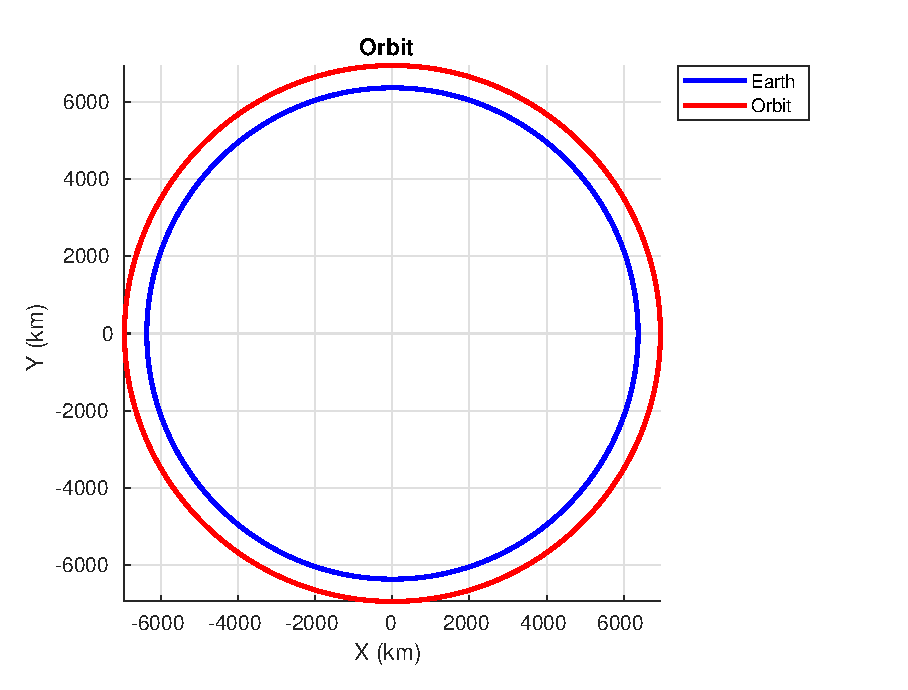
\includegraphics[width=\textwidth]{Figures/Orbit_Circular.eps}
         \caption{2D Model of the Orbit}
         \label{fig:Orbit_Circ}
     \end{subfigure}
     \hfill
     \begin{subfigure}[b]{0.45\textwidth}
         \centering
         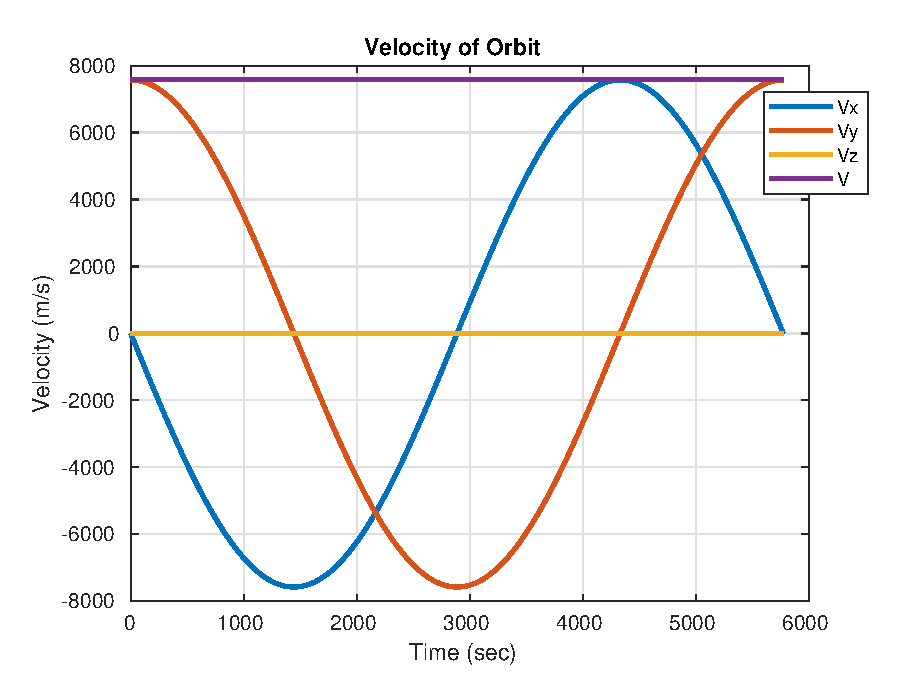
\includegraphics[width=\textwidth]{Figures/Velocity.eps}
         \caption{Velocity}
         \label{fig:Orbit_Para}
     \end{subfigure}
        \caption{Orbit Models from Analysis Tool}
        \label{fig:Orbit_Models}
\end{figure}

Initially, the elliptic orbit caused the disturbance torques to be non-uniform. In this case the only variation throughout the orbit is the magnetic field. Everything else is held constant. The analysis tool shows how the magnetic field strength changes in the orbit and can be seen in Figure \ref{fig:Mag_Models}. Figure \ref{fig:Mag_Alt} shows the magnetorquer strength as a function of time while Figure \ref{fig:Mag_Time} shows the magnetic field strength as a function of time. In this case the magnetic moment is 0.6 $A-m^2$. 

\begin{figure}[H]
     \centering
     \begin{subfigure}[b]{0.45\textwidth}
         \centering
         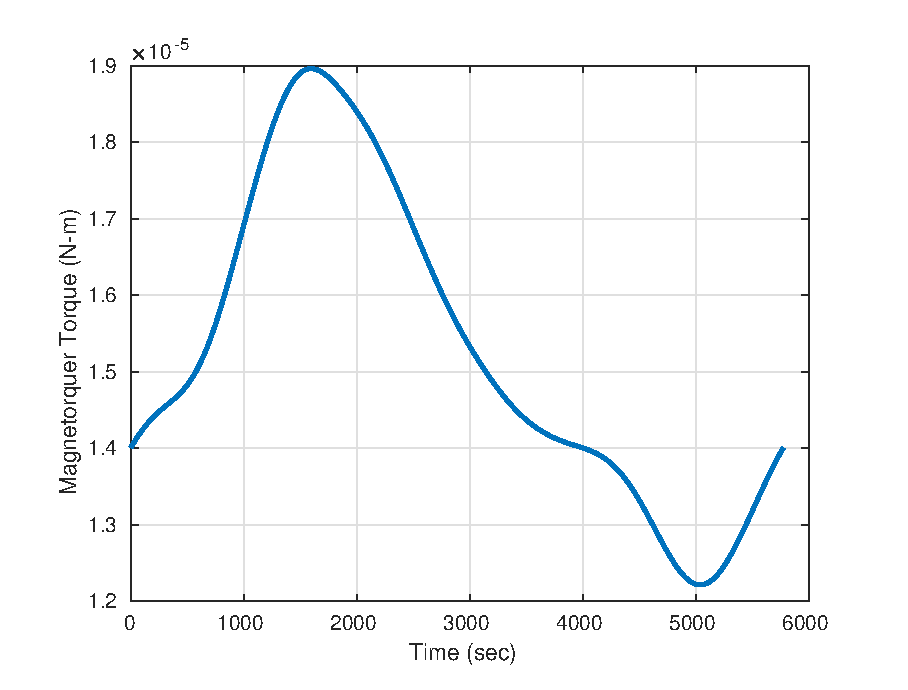
\includegraphics[width=\textwidth]{Figures/MagTorque.eps}
         \caption{Magnetorquer Torque versus Time}
         \label{fig:Mag_Alt}
     \end{subfigure}
     \hfill
     \begin{subfigure}[b]{0.45\textwidth}
         \centering
         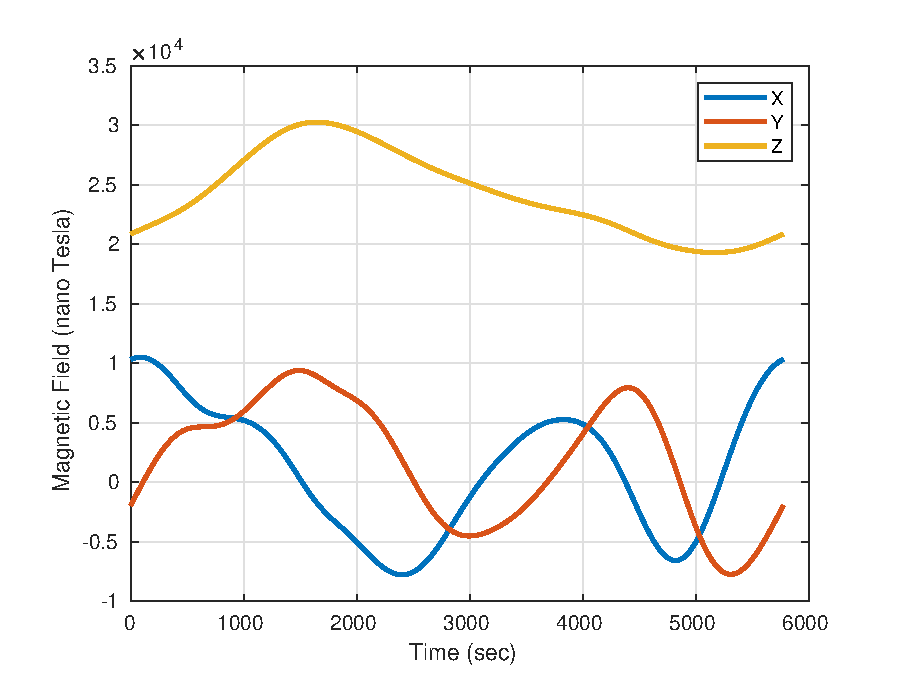
\includegraphics[width=\textwidth]{Figures/MagField.eps}
         \caption{Magnetic Field Strength versus Time}
         \label{fig:Mag_Time}
     \end{subfigure}
        \caption{Magnetic Field Strength Models from Analysis Tool}
        \label{fig:Mag_Models}
\end{figure}

After the analysis tool has modeled both the orbit and magnetic field strength, then the disturbance torques acting on the satellite during one orbit are calculated. All of the disturbance torques are then added together to get a total disturbance torque which can be seen in Figure \ref{fig:Dist_Tor} where the y-axis is plotted as a logarithm so as to see the disturbances better. 
\begin{figure}[H]
\begin{center}
    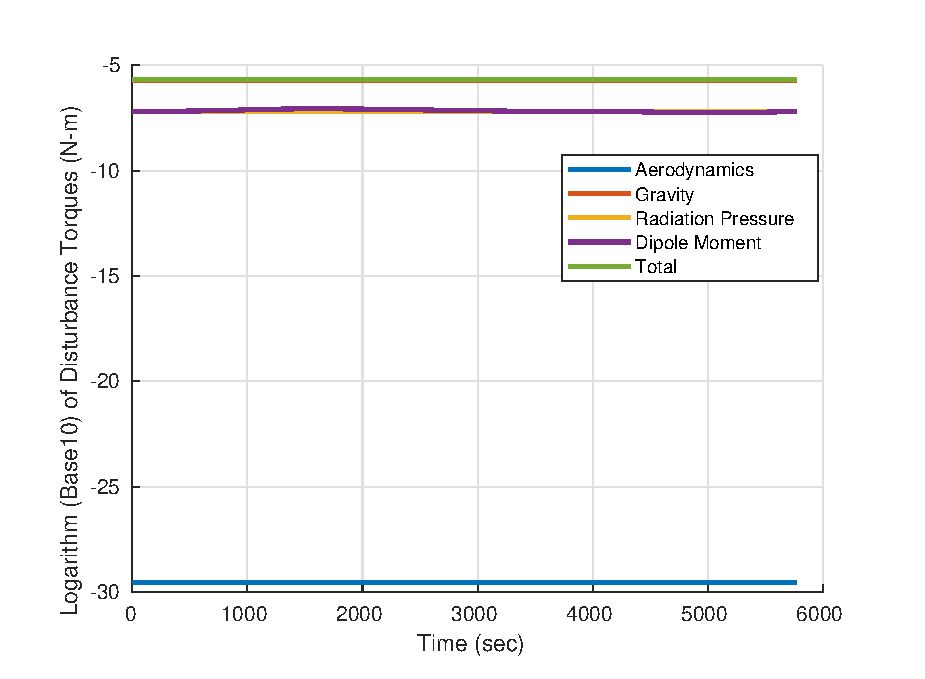
\includegraphics[width=0.8\textwidth]{Figures/Disturbances.eps}
    \caption{Logarithm of Disturbance Torques as a function of Time}
    \label{fig:Dist_Tor}
\end{center}
\end{figure}
At 600 km above the surface the aerodynamic disturbance is much lower than all other sources. In this case the total disturbances equate to a total momentum build up of 0.012261 N-m-s per orbit. Assuming an an inertia of [0.507,0.441,0.332] kg.m$^{2}$ and a maximum angular velocity of 10 deg/s the initial angular momentum in the satellite is given by [0.17456 0.15456 0.124287] $N-m-s$ along each axis respectively. Using the magnetorquers, the total momentum that can be removed from the satellite is 0.088184 N-m-s. Taking that value and substracting the disturbance torques yields a lower bound of [2.41 2.10 1.58] total orbits to detumble assuming maximum current throughout the orbit and constant 90 degree angle between the magnetorquers and the magnetic field. Due to the fact that the satellite is constantly in low orbit the magnetorquers are always effective. This would not be the case for an elliptic orbit, but in this case, reaction wheels can just be used for pointing rather than detumbling. If the reaction wheels saturate, the magnetorquers can easily be used to detumble. Due to the benign requirements for the reaction wheels, the X-ACT 100 mN-m-s system from Blue Canyon Technologies\cite{RWP500}. Using the same formula, the number of orbits used to desaturate the reaction wheels is computed as 1.3171. The only downside to using reaction wheels with only 0.1 N-m-s of storage is that the reaction wheels saturate in 8.1562 orbits. Given the period of the orbit this results in the reaction wheels saturating once a day. This of course means that the magnetorquers will need to be running all day to remove momentum while reaction wheels are used for fine pointing requirements.   

A first order analysis was performed on the control law using momentum transfer. Control using momentum transfer consists of two phases. The first phase keeps the pitch rate constant while using feedback linearization to control the roll rate through the yaw rate. The second phase reduces pitch rate and yaw rate to zero using a two axis thruster. The first order analysis consisted of two cases. The first case was applying control using momentum transfer with a diagonal inertia matrix, and the second case was applying control using momentum transfer with a non-diagonal inertia matrix. The results for using the diagonal inertia matrix can be seen in Figure \ref{fig:Diagonal_Inertia}. The first phase of the control law can be seen happening from 0 to 700 seconds. The pitch rate is held constant and the roll rate is reduced to zero as seen in Figure \ref{fig:Diagonal_Roll}. From 700 seconds till 1000 seconds, the second phase happens, and the pitch and yaw rate are both reduced to zero as seen in Figure \ref{fig:Diagonal_Pitch} and Figure \ref{fig:Diagonal_Yaw}. Despite the roll rate being reduced to zero, it does not stay at zero and immediately increases again. This is because of the diagonal inertia matrix. 

\begin{figure}[H]
     \centering
     \begin{subfigure}[b]{0.3\textwidth}
         \centering
         \includegraphics[width=\textwidth]{Figures/2StageControl/Roll_Diaganol_Matrix.png}
         \caption{Roll Rate}
         \label{fig:Diagonal_Roll}
     \end{subfigure}
     \hfill
     \begin{subfigure}[b]{0.3\textwidth}
         \centering
         \includegraphics[width=\textwidth]{Figures/2StageControl/Pitch_Diaganol_Matrix.png}
         \caption{Pitch Rate}
         \label{fig:Diagonal_Pitch}
     \end{subfigure}
     \hfill
     \begin{subfigure}[b]{0.3\textwidth}
         \centering
         \includegraphics[width=\textwidth]{Figures/2StageControl/Yaw_Diaganol_Matrix.png}
         \caption{Yaw Rate}
         \label{fig:Diagonal_Yaw}
     \end{subfigure}
        \caption{Control using Momentum Transfer with a Diagonal Inertia Matrix}
        \label{fig:Diagonal_Inertia}
\end{figure}

\noindent The results for using the non-diagonal inertia matrix can be seen in Figure \ref{fig:NonDiagonal_Inertia} where I$_{xy}$ is not zero. The first phase of the control law can be seen happening from 0 to 200 seconds. The pitch rate is held constant and the roll rate is reduced to zero as seen in Figure \ref{fig:NonDiagonal_Roll}. From 200 seconds till 1000 seconds, the second phase happens, and the pitch and yaw rate are both reduced to zero as seen in Figure \ref{fig:NonDiagonal_Pitch} and Figure \ref{fig:NonDiagonal_Yaw}. In contrast to the diagonal matrix, control using momentum transfer with the non-diagonal inertia matrix reduces the roll rate to zero and keeps it at zero. This is done because of the I$_{xy}$ being non-zero. 

\begin{figure}[H]
     \centering
     \begin{subfigure}[b]{0.3\textwidth}
         \centering
         \includegraphics[width=\textwidth]{Figures/2StageControl/Roll_NonDiaganol.png}
         \caption{Roll Rate}
         \label{fig:NonDiagonal_Roll}
     \end{subfigure}
     \hfill
     \begin{subfigure}[b]{0.3\textwidth}
         \centering
         \includegraphics[width=\textwidth]{Figures/2StageControl/Pitch_NonDiaganol.png}
         \caption{Pitch Rate}
         \label{fig:NonDiagonal_Pitch}
     \end{subfigure}
     \hfill
     \begin{subfigure}[b]{0.3\textwidth}
         \centering
         \includegraphics[width=\textwidth]{Figures/2StageControl/Yaw_NonDiaganol.png}
         \caption{Yaw Rate}
         \label{fig:NonDiagonal_Yaw}
     \end{subfigure}
        \caption{Control using Momentum Transfer with a Non-Diagonal Inertia Matrix}
        \label{fig:NonDiagonal_Inertia}
\end{figure}

\subsection{Reaction Control Systems}
Reaction Control Systems (RCS) are useful for controlling the satellite as well as desaturating reaction wheels. The downside is that they require a lot of power and volume. It also increases the weight of the spacecraft because fuel needs to be stored on the spacecraft. After an initial trade study, it was found that the RCS required too much power, failing to fit within the power requirement which was to have a total of 10 watts or less of power used by the GNC subsystem. 

%Table \ref{t:RCS} shows some of the options considered in the initial trade study.

%\begin{table}[H]
 %\centering
 %\caption{Reaction Control System Options}
 %\begin{tabular}[t]{|c|c|c|c|c|}
 %   \hline
 %   \textbf{Model Number} & \textbf{Manufacturer} & %\textbf{Mass (kg)} & \textbf{Volume (U)} & %\textbf{Power (W)} \\
 %   \hline
 %   Nano R$^3$ \cite{Enpulsion}& ENPULSION& 0.90& %0.925& 40\\
 %   \hline
 %   BGT-X5 \cite{Busek}& Busek& 1.50& 1.000& 20\\
 %   \hline
 %   FPPT (1U) \cite{CUAerospace}& CU Aerospace& %1.54& 1.000& 48\\
 %   \hline
%\end{tabular}
%\label{t:RCS}
%\end{table}

\subsection{Gimbaled Thruster}
The main form of propulsion for the satellite was to be a main thruster located on one of the faces of the satellite. The main thruster for the satellite was chosen by the propulsion team located at Auburn University. Once the orbit was changed from a highly elliptic orbit to a circular orbit in LEO the propulsion system was removed. 

%\subsection{Interface Diagrams}
%Below are the interface diagrams for the attitude control algorithm. The interface diagrams in Figure \ref{fig:AC_ID} show the components of the system and the inputs and outputs from each component. The interface diagrams are also good at showing redundancy in the option itself with Figure \ref{fig:AC_Option1} being the most redundant. Figure \ref{fig:AC_Option2} and Figure \ref{fig:AC_Option3} show viable options for attitude control but the options are less redundant than Figure \ref{fig:AC_Option1}. In this case, reaction wheels were necessary to achieve the attitude control sensitivity as defined in A.SYS.7.2. No other control mechanism (magnetorquers or gimbaled thrusters) can achieve that level of control. Thus, reaction wheels are included in each design. Magnetorquers were only considerd once the analysis tool revealed that large enough torque rods could desaturate RWs in a few orbits. The question then becomes whether to use them at all and just use the gimbaled thruster with the novel two axis control technique or include both in the event one fails or proves not to be effective.

%\begin{figure}[H]
%     \centering
%     \begin{subfigure}[b]{0.42\textwidth}
%         \centering
%         \includegraphics[width=\textwidth]{Figures/AC_ID_1.png}
%         \caption{Attitude Control Interface \\Diagram Option 1}
%        \label{fig:AC_Option1}
%     \end{subfigure}
%     \hfill
%     \begin{subfigure}[b]{0.22\textwidth}
%         \centering
%         \includegraphics[width=\textwidth]{Figures/AC_ID_2.png}
%         \caption{Attitude Control Interface Diagram Option 2}
%         \label{fig:AC_Option2}
%     \end{subfigure}
%     \hfill
%     \begin{subfigure}[b]{0.25\textwidth}
%         \centering
%         \includegraphics[width=\textwidth]{Figures/AC_ID_3.png}
%         \caption{Attitude Control Interface Diagram Option 3}
%         \label{fig:AC_Option3}
%     \end{subfigure}
%       \caption{Attitude Control Interface Diagrams}
%        \label{fig:AC_ID}
%\end{figure}

%\begin{figure}[H]
%\begin{tabular}{ccc}
%\includegraphics[width=0.42\textwidth]{Figures/AC_ID_1.png}  & \includegraphics[width=0.3\textwidth]{Figures/AC_ID_2.png} &
%\includegraphics[width=0.25\textwidth]{Figures/AC_ID_3.png}\\
%Attitude Control  & Attitude Control & Attitude Control \\ Interface Diagram Option 1  & Interface Diagram Option 2 & Interface Diagram Option 3 \\
%\label{t:AC_ID}
%\end{tabular}
%\caption{Attitude Control Interface Diagrams}
%\label{fig:AC_ID}
%\end{figure}

%\begin{figure}[H]
%\centering
%\includegraphics[width=0.5\textwidth]{Figures/AC_ID_1.png}
%\caption{Attitude Control Interface Diagram Option 1}
%\label{fig:AC_ID_1}
%\end{figure}

%\begin{figure}[H]
%\centering
%\includegraphics[width=0.4\textwidth]{Figures/AC_ID_2.png}
%\caption{Attitude Control Interface Diagram Option 2}
%\label{fig:AC_ID_2}
%\end{figure}

%\begin{figure}[H]
%\centering
%\includegraphics[width=0.3\textwidth]{Figures/AC_ID_3.png}
%\caption{Attitude Control Interface Diagram Option 3}
%\label{fig:AC_ID_3}
%\end{figure}

%The inputs and outputs for the Attitude Control IDs differ between each option due to the components that make up each option. In each option, the hardware components being considered are marked with gray boxes, and clear boxes mark components not considered by GNC. The gimbal thruster and magnetorquers only take inputs from the ADCS board. The gimbaled thruster takes on on/off signal and thruster direction, and the magnetorquer receives current from the ADCS Board. The reaction wheels have both an input and output. The reaction wheels receive a signal to spin up from the ADCS Board and output the angular velocity of the reaction wheel to track the momentum storage. 

\subsection{Tradeoffs and Considerations}
Throughout the design process of the satellite, redundancy is always a primary consideration, but especially so here. Without proper attitude control, disturbance torques will overcome the orientation of the system and prevent the mission from being successful. The team must also consider, where in the orbit different control mechanism are effective. A TPM Update showing the mass, power, and volume was found for the attitude control subsystem. Table \ref{t:AC_TPM_Update3} shows the minimum, average, and maximum values for the power, mass, and volume of the subsystem. 

%for Figure \ref{fig:AC_Option1}. Table \ref{t:AC_TPM_Update2} shows the minimum, average, and maximum values for the power, mass, and volume for Figure \ref{fig:AC_Option2}. Lastly, Table \ref{t:AC_TPM_Update3} shows the minimum, average, and maximum values for the power, mass, and volume for Figure \ref{fig:AC_Option3}. Note that Table \ref{t:AC_TPM_Update1} and Table \ref{t:AC_TPM_Update3} are the same because the components that were analyzed for the TPM updated are the same.

%\begin{table}[H]
% \centering
% \caption{Attitude Control TPM Update 1}
%\begin{tabular}{ |c|c|c|c|  }
% \hline
% \textbf{TPM} & \textbf{Min} & \textbf{Avg} & %\textbf{Max} \\
% \hline
% \textbf{Power [W]} & 2.7& 12.42& 35.25\\
% \hline
% \textbf{Mass [g]} & 172.50& 1442.79& 3522\\
% \hline
% \textbf{Volume [cm$^3$]} & 81.23& 847.30& %2585.52\\
% \hline
%\end{tabular}
%\label{t:AC_TPM_Update1}
%\end{table}%

%\begin{table}[H]
% \centering
% \caption{Attitude Control TPM Update 2 - No %Magnetorquers}
%\begin{tabular}{ |c|c|c|c|  }
% \hline
% \textbf{TPM} & \textbf{Min} & \textbf{Avg} & %\textbf{Max} \\
% \hline
% \textbf{Power [W]} & 1.95& 9.96& 30\\
% \hline
% \textbf{Mass [g]} & 150& 1309.62& 3300\\
% \hline
% \textbf{Volume [cm$^3$]} & 57.23& 767.80& 2430\\
% \hline
%\end{tabular}
%\label{t:AC_TPM_Update2}
%\end{table}

\begin{table}[H]
 \centering
 \caption{Attitude Control TPM Update}
\begin{tabular}{ |c|c|c|c|  }
 \hline
 \textbf{TPM} & \textbf{Min} & \textbf{Avg} & \textbf{Max} \\
 \hline
 \textbf{Power [W]} & 2.7& 12.42& 35.25\\
 \hline
 \textbf{Mass [g]} & 172.50& 1442.79& 3522\\
 \hline
 \textbf{Volume [cm$^3$]} & 81.23& 847.30& 2585.52\\
 \hline
\end{tabular}
\label{t:AC_TPM_Update3}
\end{table}

\subsection{Final Design Selections}
It was determined that to have appropriate number for each component the satellite would need one reaction wheel and one magnetorquer for each axis for a total of three reaction wheels and three magnetorquers. The magnetorquers are included as a fall back option in the event the two axis control law does not perform as intended and to utilize less fuel. After evaluating the tradeoffs and system requirements, it was determined that the components needed would be the NewSpace Systems NCTR-M012 \cite{M012} magnetorquers using a RS485 interface protocol and the Blue Canyon Tech for the highly elliptic orbit. RWP500 \cite{RWP500} reaction wheels use a RS422 interface protocol. From the analysis tool results, the total momentum storage for each reaction wheels based on the inertias of the satellite is 0.15 Nms. The RWP500 reaction wheel has a momentum storage of 0.5 Nms which is well above the requirement of 0.15 Nms. The RWP500 has a smaller mass, volume, and power than the Tamagawa Seiki \cite{Tamagawa-RW} and MicroWheel 200 \cite{MSCI} reaction wheels. Although there are reactions wheels closer to the required momentum storage, these reaction wheels have larger TPMs than the RWP500s which is why the RWP500s were chosen over other viable options. The Sinclair Planetary 400 mNms \cite{Sinclair-Light} reaction wheels was not chosen due to these reaction wheels still being developed by Sinclair Planetary. The analysis tool also helped with the magnetorquer sizing. The NCTR-M012 magnetorquers were chosen because these magnetorquers would desaturate the reaction wheels in 9.02 orbits. Although there are magnetorquers that can desaturate the reaction wheels quicker, the NCTR-M012 has less mass, volume, and/or power than the quicker options. \textbf{\textit{The TPM for the final design selection is as follows: 20.40 watts of power, 2409 grams of mass, and 1434.90 cubic centimeters of volume.}} Once the orbit changed however, the RWP100 were re-investigated given the effectiveness of the magnetorquers in LEO. With this configuration the RWP100's only used {\bf 1.0 watt of power, 1000 grams of mass and 367.5 cubic centimeters of volume.} This is considerably less than the initial TPM and is possible because the magnetorquers can detumble the satellite. Furthermore, it allows the option of using the XACT-100 integrated subsystem. 

%%%%%%%%%%%%%%%%%%%%%%%%%%%%%%%%%%%%%%%%%%%%%%%%%%%%%%%%%%%%%%%%%%%%%%%%%%%%%%%%%%%%%%%%%%%%%%%

\section{Position Estimation}
\subsection{Position Estimation Overview}
Position estimation is the function by which the position is determined using integration schemes, GPS, clocks and a ground station network (GSN) like the Deep Space Network (DSN) for example. During orbit, an accurate estimation of position must be known so that proper sensors, models and mechanisms may be used. The CONOPS for position estimation is shown in the following activity diagram. Figure \ref{fig:PE_AD_2} shows a generalized overview of the position estimation procedure. The procedure starts by getting an initial position coordinates from the GPS. Simultaneously, an RK4 routine is run to integrate the equations of motion of the satellite in LEO obtaining position coordinates in between GPS updates. If the GPS returns an updated valid measurement, the integration scheme is updated with these new coordinates. This process is repeated every time a GPS update or GSN update is received.

\begin{figure}[H]
\centering
\includegraphics[width=1.0\textwidth]{Figures/PE_AD_2.png}
\caption{Position Estimation Procedure}
\label{fig:PE_AD_2}
\end{figure}

\subsection{Global Positioning Systems}
The Global Positioning System (GPS) is a utility which provides users with positioning, timing, and navigation services. The benefits of using GPS tracking are that it provides position estimation,  time, and other features. The issue lies in where GPS can be used. GPS only works within a certain altitude from the Earth. The initial apogee of ABEX's orbit was 60,000 km while the GPS constellation is at 35,000 km. Thus, for large parts of the orbit, GPS would not have been a viable option. However, it was assumed that at least once per orbit (during the 20 minute perigee pass), the GPS would provide a valid position update for the estimation algorithm. The GPS unit to be used was initially tasked to ADCS, but was eventually selected by the Communications team. The GPS receiver chosen was the SparkFun GP-20U7 which comes with a customizable interface protocol. This GPS receiver is a 56-channel GPS module that supports a standard NMEA-0183 and uBlox 7 protocol. To have redundancy in the system, four GPS Receivers will be put on the satellite. Once the orbit changed to LEO, the issue with being within the GPS constallation was no longer a problem.

\subsection{Ground Station Network}
The Communication subsystem team was tasked with determining the best method to communicate with ground personnel. It is assumed that two way communication will be possible and that at least one way communication will be utilized. Typically Ground Station Networks (GSNs) are used to communicate with satellites with the Deep Space Network (DSN) being the most well known. These GSNs are capable of sending a state vector to the satellite to update its estimate of the model. With so many active satellites in space however, it is often difficult to obtain "radio" time on these networks to communicate with a specific satellite. As such, it can only be assumed that state vector updates from a GSN will happen intermittently and is not a guarantee. As such an integration scheme is used as explained in the next section.

\subsection{Integration Scheme}
As explained above, GPS and any communication with GSNs will only update a few times per orbit. As such, an integration schemes must be used to predict the path that the spacecraft in between GPS and GSN updates. One such integration scheme is the Runge-Kutta method, which is used to construct high accuracy models of functions, without requiring the high order derivatives of the functions. It was suggested that the use of an RK4 method for this application would be the best option and was thus chosen for this design. In this case, in between GPS and GSN updates, a nonlinear gravity field model will be used to integrate the position vector over time. The model states and sensor update states will be fused using a standard Kalman Filter approach \cite{kalman}. 

%\subsection{Interface Diagrams}
%Below are the interface diagrams for the position estimation algorithm. The interface diagrams show the components of the system and the inputs and outputs from each component. The interface diagrams in Figure \ref{fig:PE_ID} are also good at showing redundancy in the option itself with Figure \ref{fig:PE_Option1} being the most redundant. Figure \ref{fig:PE_Option2} and Figure \ref{fig:PE_Option3} show viable options for position estimation, but the options are less redundant than Figure \ref{fig:PE_Option1}. 

%\begin{figure}[H]
%%     \centering
%     \begin{subfigure}[b]{0.5\textwidth}
%         \centering
%         \includegraphics[width=\textwidth]{Figures/PE_ID_1.png}
%         \caption{Position Estimation Interface Diagram Option 1}
%         \label{fig:PE_Option1}
%     \end{subfigure}
%     \hfill
%     \begin{subfigure}[b]{0.42\textwidth}
%         \centering
%         \includegraphics[width=\textwidth]{Figures/PE_ID_2.png}
%         \caption{Position Estimation Interface Diagram Option 2}
%         \label{fig:PE_Option2}
%     \end{subfigure}
%     \hfill
%     \begin{subfigure}[b]{0.55\textwidth}
%         \centering
%         \includegraphics[width=\textwidth]{Figures/PE_ID_3.png}
%         \caption{Position Estimation Interface Diagram Option 3}
%         \label{fig:PE_Option3}
%     \end{subfigure}
%        \caption{Position Estimation Interface Diagrams}
%        \label{fig:PE_ID}
%\end{figure}

%\begin{figure}[H]
%\begin{tabular}{cc}
%\includegraphics[width=0.4\textwidth]{Figures/PE_ID_1.png} & \includegraphics[width=0.4\textwidth]{Figures/PE_ID_2.png} \\
%Position Estimation &  Position Estimation \\ Interface Diagram Option 1 & Interface Diagram Option 2 \\ \\
%\includegraphics[width=0.4\textwidth]{Figures/PE_ID_3.png} & \\
%Position Estimation \\ Interface Diagram Option 3 \\
%\label{t:PE_ID_1}
%\end{tabular}
%\caption{Position Estimation Interface Diagrams}
%\label{fig:PE_ID}
%\end{figure}


%The inputs and outputs for the Position Estimation IDs differ between each option due to the components that make up each option. In each option, the hardware components being considered are marked with gray boxes, and clear boxes mark software components and hardware components not considered by GNC. In this case, all hardware is being considered by other teams and only the algorithm is being considered. The requirement for 1000 km knowledge necessitates the need for an RK11 integration loop. GPS and any GSN do not update fast enough to obtain that kind of precision. Thus, in between sensor updates, the position will need to be estimated using the RK11 algorithm. However, it may be possible to only use GSN or GPS and not both. 
%The input to the Real Time Clock and the GPS receiver is power from the ADCS Board. The output from the Real Time Clock is time, and the outputs of the GPS receiver are altitude, longitude, latitude, velocity, and GPS time. The input to the RK11 integration loop algorithm is the coordinates of the satellite from the ADCS Board, and the output from the RK11 integration loop algorithm is the time-updated coordinates of the satellite. Finally, the ADCS Board receives an output from the communication board. This output is range data that will be received from a GSN that can be used to obtain current position. 

\subsection{Tradeoffs and Considerations}
As with the other functions under the GNC team, position estimation requires redundancy. If the satellite loses track of its position in orbit, sensors cannot be used at the proper times, desaturation could become impossible, and the mission would fail altogether. The biggest consideration to make is where each solution works. For instance, as stated before, GPS only works within a certain altitude from the Earth. Therefore, the mission could not rely solely on GPS for position estimation since the satellite was to be traveling on a hybrid orbit between LEO and HEO. Once the orbit changed to only LEO this was no longer an issue. As such the hybrid GPS, GSN, RK4 method satisfies all constraints. In addition, the XACT-100 from BCT can also integrate this a GPS using a multi-pin connector.  

%A trade study was performed to find the best combination of components for the Position Estimation. The trade study was driven by the power, mass, and volume requirements. A TPM Update showing the mass, power, and volume was found for each interface diagram. Table \ref{t:TPM_Update3} shows the minimum, average, and maximum power, mass, and volume for the Figure \ref{fig:PE_Option1} and Figure \ref{fig:PE_Option3}. Since Figure \ref{fig:PE_Option2} does not contain any components of interest to the GNC Team, a TPM Update was not made.

%\begin{table}[H]
%\centering
% \caption{Position Estimation TPM Update}
%\begin{tabular}{ |c|c|c|c|  }
% \hline
% \textbf{TPM} & \textbf{Min} & \textbf{Avg} & %\textbf{Max} \\
% \hline
% \textbf{Power [W]} & 0.50 & 1.32 & 2.50 \\
% \hline
% \textbf{Mass [g]} & 45 & 109.72 & 167 \\
% \hline
% \textbf{Volume [cm$^3$]} & 70 & 126.21 & 1730 \\
% \hline
%\end{tabular}
%\label{t:TPM_Update3}
%\end{table}

\subsection{Final Design Selections}
The Communication subsystem and Control and Data Handling subsystem dealt with all of the hardware components shown in the BDD for Position Estimation. As such, only the overall CONOPS and BDDs were designed by ADCS. In addition, the XACT-100 would house a GPS and flight control board capable of position estimation that satisfies the systems engineering requirements. 

%\textbf{\textit{The TPM Update for the final design selection is as follows: 0.53 W of power, 40 g of mass, and 1.36 cm$^3$ of volume. However, after discussing with subject matter experts, there are concerns over the effectiveness of the GP-20U7. Further analysis will be necessary.}}

%%%%%%%%%%%%%%%%%%%%%%%%%%%%%%%%%%%%%%%%%%%%%%%%%%%%%%%%%%%%%%%%%%%%%%%%%%%%%%%%%%%%%%%%%%%%%%%

\section{Risk Considerations}
There is a plethora of risks to consider with the GNC of this mission. Fortunately, for most of these risks, there are effective mitigation strategies that can be implemented. Also, if the mitigation strategies fail, redundancies have been put in place to maintain the function of the mission, should a component fail completely. The risk considerations and mitigation tactics have been outlined in Table \ref{t:Risks1}. In addition to these risks outlined below, a risk criticality matrix has also been created (Table \ref{t:RISK_MATRIX}). Notice that only 4 risks are in yellow region. These 4 risks include procuring hardware due to supply chain delays, an inadequate labor force due to a large drop in student enrollment and rate gyro drift and vibrations in the structure. The last two though have been mitigated since the change in orbit because the XACT-100 has flight heritage and thus will have mitigated the rate gyro drift issue and has also already survived numerous missions undergoing travel and launch vibrations. 

\begin{center}
\begin{longtable}[c]{|c|c|p{4.0cm}<{\centering}|p{4.0cm}<{\centering}|}
\caption{Risk Considerations} \label{t:Risks1} \\

\hline \rowcolor{cyan} \multicolumn{1}{|c|}{\textbf{ID}} & \multicolumn{1}{c|}{\textbf{Title}} & \multicolumn{1}{c|}{\textbf{Statement}} & \multicolumn{1}{c|}{\textbf{Current Handling Strategy}} \\ \hline 
\endfirsthead

\multicolumn{4}{c}%
{{\bfseries \tablename\ \thetable{} -- Continued from previous page}} \\
\hline \rowcolor{cyan} \multicolumn{1}{|c|}{\textbf{ID}} & \multicolumn{1}{c|}{\textbf{Title}} & \multicolumn{1}{c|}{\textbf{Statement}} & \multicolumn{1}{c|}{\textbf{Current Handling Strategy}} \\ \hline 
\endhead

\hline \rowcolor{cyan} \multicolumn{4}{|r|}{{\textbf{Continued on next page}}} \\ \hline
\endfoot

\hline \hline
\endlastfoot

1  & Electrical Components & Given that space contains numerous radioactive particles, there is a possibility of particles impacting circuitry adversely impacting electronics in the ADCS system, which can result in loss of ADCS effectiveness. & Mitigation strategies include pre-flight inspection of reaction wheel bearings and sufficient redundancy within the subsystem. \\ \hline 
\rowcolor{lightgray} 2  &  Vibrations & Given that vehicle launches cause mechanical disturbances, there is a possibility of vibrations and g-forces adversely impacting all components in the ADCS system, which can result in loss of ADCS effectiveness. & Mitigation strategies include pre-launch tests to ensure security against vibrations and g-forces. \\ \hline 
3  &  Magnetorquers & Given that another magnetic field may be present, there is a possibility of magnetic field interference adversely impacting the magnetorquer(s), which can result in loss of control of the magnetorquers. & Mitigation strategies include ample separation from any other components that may produce a magnetic field. \\ \hline 
\rowcolor{lightgray} 4  &  Reaction Wheels & Given that the reaction wheels have sensitive bearings, there is a possibility of electrostatic discharge from space weather effects such as coronal mass ejections adversely impacting the smoothness of the reaction wheel bearings, which can result in a loss of attitude control. & Mitigation strategies include discussing potential mitigation strategies with BCT about their XACT-100 RWs. \\ \hline 
5  &  Rate Gyro 3DOF & Given that biases in data exist, there is a possibility of drift in the integration schemes adversely impacting the attitude determination algorithm, which can result in a loss of attitude knowledge. & Mitigation strategies include a Kalman Filter which will correct errors due to biases. \\ \hline 
\rowcolor{lightgray} 6  &  Magnetometer & Given that the structure and magnetorquers may produce additional magnetic fields, there is a possibility of magnetic field interference adversely impacting the magnetometer, which can result in inadequate attitude control using magnetorquers and attitude estimation in the event the star tracker is not operational. & Mitigation strategies include ample separation from any other components that may produce a magnetic field. \\ \hline 
7  &  Star Trackers & Given that the sun occupies a large portion of the FOV, there is a possibility of light saturation of the star tracker adversely impacting attitude determination algorithm, which can result in loss of attitude knowledge in the event that the magnetometers and sun sensors are not operational. & Mitigation strategies include a baffle for reduction of stray light coming in the vicinity of the star tracker lens. In the case where this failure occurs, the star tracker’s attitude estimation functions would be sent to other sensors such as a sun sensor with a magnetometer. \\ \hline 
\rowcolor{lightgray} 8  &  Sun Sensors & Given that numerous sources of light in space exist, there is a possibility of light interference adversely impacting the sun sensor, which can result in inaccuracies in attitude estimation in the event the star tracker is not operational. & Mitigation strategies include a baffle for reduction of stray light coming in the vicinity of the star tracker lens. \\ \hline 
9  &  GPS Receiver & Given that there are a variety of signals travelling from different sources in space, there is a possibility of GPS interference from man made sources such as other satellites adversely impacting the position estimation algorithm, which can result in a loss of position knowledge. & Mitigation strategies include following spectrum regulations to minimize interference. \\ \hline 
\rowcolor{lightgray} 10 &  GPS Receiver & Given that there are a variety of signals travelling from different sources in space, there is a possibility of GPS interference from natural sources such as solar flares adversely impacting the position estimation algorithm, which can result in a loss of position knowledge. & Mitigation strategies include enclosing vital electronics in metal shielding to protect from interference from natural sources. \\ \hline 
11 &  Inadequate Labor Force & Given that the writing and debugging of software is tedious and time consuming, there is a possibility of inadequate labor allocation adversely impacting the timeline of the mission, which can result in an overall delay of the mission. & Mitigation strategies include ensuring deadlines are being met on time and providing funding for the appropriate amount of student assistance on the project. \\ \hline 
\rowcolor{lightgray} 12 &  Procuring Hardware & Given that production around the world has been slowed for over a year now, there is a possibility of lead times on procuring hardware adversely impacting the timeline of the mission, which can result in the overall delay of the mission. & Mitigation strategies include identifying hardware that is desired early on to ensure ample time to procure it for when it is needed. \\
\end{longtable}
\end{center}

\begin{table}[H]
 \centering
 \caption{Risk Matrix for GNC Subsystem}
\begin{tabular}{|c|c|c|c|c|c|c|}
 \hline
  &  & \multicolumn{5}{c|}{Risk Criticality Matrix} \\
 \hline
 5 & \multirow{5}{*}{\rotatebox{90}{\textbf{Likelihood}}} & \cellcolor{green} & \cellcolor{yellow} & \cellcolor{red} & \cellcolor{red} & \cellcolor{red} \\\cline{1-1}\cline{3-7}
 4 &  & \cellcolor{green} & \cellcolor{yellow} & \cellcolor{yellow} & \cellcolor{red} & \cellcolor{red} \\\cline{1-1}\cline{3-7}
 3 &  & \cellcolor{green} & \cellcolor{green} 1,3,6,9,10 & \cellcolor{yellow} 2,5,11 & \cellcolor{yellow} 12 & \cellcolor{red} \\\cline{1-1}\cline{3-7}
 2 &  & \cellcolor{green} & \cellcolor{green} 7,8 & \cellcolor{yellow} & \cellcolor{yellow} & \cellcolor{yellow} \\\cline{1-1}\cline{3-7}
 1 &  & \cellcolor{green} & \cellcolor{green} & \cellcolor{green} & \cellcolor{green} & \cellcolor{yellow} \\\cline{1-1}\cline{3-7}
 \hline
  &  & \multicolumn{5}{c|}{\textbf{Consequence}} \\
 \hline
  &  & 1 & 2 & 3 & 4 & 5 \\
 \hline
\end{tabular}
\label{t:RISK_MATRIX}
\end{table}

%%%%%%%%%%%%%%%%%%%%%%%%%%%%%%%%%%%%%%%%%%%%%%%%%%%%%%%%%%%%%%%%%%%%%%%%%%%%%%%%%%%%%%%%%%%%%%%

\section{Conclusion}
The mission requirements presented have been partially fulfilled, as shown in Table \ref{t:SYS_REQ} while carefully considering potential risks with each option. System constraints  were trickled down to subsystem requirements and constraints. The requirements were split into Attitude Estimation, Attitude Control and Position Estimation requirements to ease design. Several solutions were considered for each of these major functions. 

The Attitude Estimation solution is to utilize two IMUs in conjunction with a star tracker, six sun sensors and two magnetometers. This allows for ample redundancy, ensuring that the satellite can operate despite component failure. The solution for position estimation is the inclusion of four GPS receivers, which ensures redundancy in conjunction with updates from GSN and an RK4 integration routine to obtain state updates between sensor updates. A novel solution for attitude control was presented although it may not be necessary given the change in orbit. A combination of three magnetorquers and three reaction wheels are used for attitude control. This entire GNC system defined above is to be housed in the XACT-100 system from BCT. 

%Additionally, solutions to GNC problems yield their own issues. One such issue is that of utilizing magnetic fields and potential interference. Many solution options include hardware which uses magnetic field data to achieve position or attitude estimation and attitude control. This data can be rendered inaccurate or nonexistent by interference from a magnetic field different from Earth’s or being outside of the proximity of Earth’s magnetic field entirely. To solve this issue, the system will use other means of estimation or control such as reaction wheels instead of magnetorquers for desaturation, while outside of Earth’s magnetic field. A number of issues like this arose and were considered during the final design selections for the system functions. Another consideration the team had is risk factors. Risk factors also play a significant role in the selection of design, solutions and hardware. 

The team’s risk considerations have been outlined as well as mitigation strategies as shown in Table \ref{t:Risks1}. The most notable of these risks is the failure of hardware due to circumstances out of the control of the mission and the interference from outside sources to functions such as attitude control. The team proposed mitigation strategies to these risks including separation between any parts that may interfere with one another and ample redundancy such as more than three reaction wheels. Final design solutions have been selected to satisfy all mass, volume and power requirements, as well as accuracy requirements such as location accuracy and attitude knowledge, as well as mitigate any possible risks identified by the team to ensure the success of the mission.

%%%%%%%%%%%%%%%%%%%%%%%%%%%%%%%%%%%%%%%%%%%%%%%%%%%%%%%%%%%%%%%%%%%%%%%%%%%%%%%%%%%%%%%%%%%%%%%

\section*{Acknowledgments}
We would like to acknowledge the multiple other teams that have been working hard to design this satellite. Without their help and expertise in the different subsystems, this satellite would not have proceeded as smoothly as it has. We would also like to acknowledge the System Engineering Management Team: Michael Halvorson, Jared Fuchs, and Victor Lopez.

%%%%%%%%%%%%%%%%%%%%%%%%%%%%%%%%%%%%%%%%%%%%%%%%%%%%%%%%%%%%%%%%%%%%%%%%%%%%%%%%%%%%%%%%%%%%%%%

\bibliography{sample}
\end{document}